%\section{Droplet deformation in stokestain dilute emulsions}
\section{Averaged equations for dispersed fluid-fluid flows with surface tension}%Newtonian dispersed two-phase flows with constant surface tension and no interfacial transfer}
\label{sec:averaged_surface}

%We now consider a dilute mono-disperse suspension of spherical droplet of radius $a$ without mass transfer. 
%The dispersed  and continuous phases are considered Newtonian fluids defined by the constant viscosities $\mu_k$ and density $\rho_k$.
%Additionally, the surface tension coefficient at the interface between both fluids is noted $\gamma$. 
%Because we consider a small droplet Reynolds number, we assert that only the averaged mass and momentum equations are sufficient to describe the mixture. 

We consider a monodisperse fluid-fluid suspension of droplets (or bubbles) which are not necessarily spherical with volume \( v_p \), in the absence of mass transfer. 
Both the dispersed and continuous phases are treated as incompressible Newtonian fluids, characterized by constant viscosities \( \mu_k \) and densities \( \rho_k \). 
The surface tension at the interface between the two fluids is denoted by \( \gamma \) which is not necessarily constant.%and is not a constant although we do not specify yet its .
%Although we do not specify the % and is  to be constant. 
%\JL{je ne pense pas que c'est necessaire de supposer que la tension de surface est constante ici}
We only consider in the next section averaged mass and momentum conservation equations to describe the motions of the phases. 
% \JL{tu dis cela car on ne consideres pas lenergie cinetique ?}
\begin{table}
    \centering
    \begin{tabular}{|c|ccl|}\hline
    & Conservation law & mass & momentum \\ \hline
    Conserved quantity & $f_k^0$  & $\rho_k$ & $\rho_k \textbf{u}_k^0$ \\
    Source term & $s_k^0$  & $0$ & $\rho_k \textbf{g}$ \\
    Diffusive flux & $\Phi_k^0$ & 0 & $\bm\sigma_k^0 = -p_k^0 + \mu_k (\grad \textbf{u}_k^0 + \grad \textbf{u}_k^0)$ \\
    Surface diffusive flux & $\Phi_\Gamma^0$ & 0 & $\bm\sigma_\Gamma^0 = \gamma (\bm\delta - \textbf{nn})$ \\\hline
    \end{tabular}

    \caption{Definition of the physical quantities and local constitutive laws for phases $k$.}
    \label{tab:qte_Newtonian}
\end{table}
The conserved physical quantities  relevant to the problem are summarized in Table \ref{tab:qte_Newtonian}.


In the following, we consider the influence of Marangoni effects on the suspension dynamics. Surfactants and/or non-uniform temperature gradients typically cause variations in the surface tension coefficient at the droplet interfaces. 
One must solve a transport equation for either the temperature field or the surfactant concentration in order to determine the proper surface tension distribution on the droplet surface \citep{Subramanian_1985,leal2007advanced}. 
This can be done using the surface transport equations derived in \ref{sec:local_eq}. 
However, as these complexities fall outside the scope of this work, we assume that the surface tension coefficient is known in advance, having been determined from a separate problem solved a priori.



After presenting the higher-order mass and momentum moments required to describe the particle rotation and deformation we derive the averaged equations for mass, momentum and first moment of momentum for a fluid-fluid suspension.
The presentation is inspired by \citep{lhuillier2009rheology}, while extending it beyond the scope of solid particles.
Then we turn to the decomposition of stress within the moment formulation. 
The section concludes with a discussion of the symmetry properties of the effective stress tensor, employing arguments analogous to those presented by \citet{lhuillier1996contribution}.
%We finalize the section with a discussion on the symmetry of the effective stress tensor using arguments similar to \citep{lhuillier1996contribution}.

%In summary, we deal with the exact same scenario as 
%\citet[Appendix B]{zhang1997momentum}, i.e. dilute mono-disperse emulsion of inertialess droplets. 
%The goal of this section is not to demonstrate any new physical phenomenon, but rather to explain what is the meaning of the higher moment equations in this simple context, how they can be used to determine the droplets shapes, and how they are connected to the continuous phase averaged equations. 


\subsection{Higher-order mass and momentum moments}


% \tb{peut etre mettre les equaitons fluid non-moyenne}

%Note that $\textbf{M}_\alpha$ is analogous to the inertia tensor $\textbf{I}_\alpha$ in solid mechanics, $\textbf{M}_\alpha$ and $\textbf{I}_\alpha$ are related through the expression $\textbf{I}_\alpha = (\bm\delta : \textbf{M}_\alpha)\bm\delta - \textbf{M}_\alpha$.
%For a fluid with a constant density, the tensor $\textbf{M}_\alpha$ describes the second moment of the volume distribution around the particle center of mass.
%Likewise, the tensor $\textbf{P}_\alpha$ describes the first moment of the velocity distribution within the particle volume. 
%To provide a clearer physical interpretation of the moment of momentum tensor, we decompose $\textbf{P}_\alpha$ into three distinct parts, denoted as $\textbf{S}_\alpha$, $\textbf{T}_\alpha$ and $P_\alpha$ such that,
%$\textbf{P}_\alpha = \textbf{S}_\alpha+\textbf{T}_\alpha + P_\alpha\bm\delta$, where $\textbf{S}_\alpha = \frac{1}{2}(\textbf{P}_\alpha + \textbf{P}_\alpha^\dagger - \frac{2}{3}(\bm\delta:\textbf{P}_\alpha)\bm\delta)$ represents the symmetric traceless part of $\textbf{S}_\alpha$ and $\textbf{T}_\alpha = \frac{1}{2}(\textbf{P}_\alpha - \textbf{P}_\alpha^\dagger)$ is the antisymmetric part of $\textbf{P}_\alpha$.
%Then, the tensors $\textbf{S}_\alpha$ and $\textbf{T}_\alpha$ correspond respectively to the stretching and angular momentum of the particle $\alpha$. 
%The tensor $\textbf{S}_\alpha$ quantifies how fast and in which direction the particle gets elongated or flattened, in other words it represents the mean rate of deformation experienced by the particle.
%The tensor $\textbf{T}_\alpha$ is related to the angular momentum of the particle denoted by the pseudo vector $\bm\mu_\alpha = \intO{ \rho_d \textbf{r} \times \textbf{u}_d^0 }$. 
%Indeed, both  $\textbf{T}_\alpha$ and $\bm{\mu}_\alpha$ represent the angular momentum and are related through $(\bm{\mu}_\alpha)_i = \epsilon_{ijk} (\textbf{T}_\alpha)_{jk} = \epsilon_{ijk} (\textbf{P}_\alpha)_{jk}$, where $\bm\epsilon$ is the third order alternating unit tensor or Levi-Cita tensor. 
%Lastly, we also introduce the scalar $P_\alpha =\frac{1}{3}\bm\delta : \textbf{P}_\alpha$, which quantifies the rate at which the particle is being compressed or expanded.
%In our case $P_\alpha =0$ because the interior velocity field of a droplet is assumed divergence free. 
%To better explain the implication of these quantities on the particle kinematics   we provide in \ref{eq:scheme}, three plots representing possible inner velocity fields with their corresponding value of the moment of momentum tensor.

To describe the dispersed phase in addition to the quantities defined in \ref{sec:Lagrangian} we define the second-order moment of mass and the first-order moment of momentum as 
\begin{equation}
    \textbf{M}_\alpha 
    = \intO{ \rho_d \textbf{r} \textbf{r} }
    \;\;\;\text{and}\;\;\;
    \textbf{P}_\alpha 
    = \intO{ \rho_d \textbf{r} \textbf{u}_d^0 },
    \label{eq:first_moment_of_momentum_def}
\end{equation}
respectively. 
Note that the tensor $\textbf{M}_\alpha$ plays a role analogous to the inertia tensor $\textbf{I}_\alpha$ in solid mechanics. 
The two are related by the expression  $\textbf{I}_\alpha = (\bm\delta : \textbf{M}_\alpha)\bm\delta - \textbf{M}_\alpha$.
For a fluid of constant density, $\textbf{M}_\alpha$ represents the second moment of the mass distribution relative to the particle center of mass.
Similarly, the tensor $\textbf{P}_\alpha$ is the first moment of the momentum distribution within the particle volume. 
To offer a clearer physical interpretation of the moment of momentum tensor, we decompose $\textbf{P}_\alpha$ into three distinct components  
\begin{equation}
\textbf{P}_\alpha = \textbf{S}_\alpha + \textbf{T}_\alpha + P_\alpha \bm\delta,
\end{equation}
where $\textbf{S}_\alpha = \frac{1}{2}\left(\textbf{P}_\alpha + \textbf{P}_\alpha^\dagger - \frac{2}{3}(\bm\delta:\textbf{P}_\alpha)\bm\delta\right)$ is the symmetric traceless part, representing the  deformation or stretching of momentum,
$\textbf{T}_\alpha = \frac{1}{2}(\textbf{P}_\alpha - \textbf{P}_\alpha^\dagger)$ is the antisymmetric part, associated with the angular momentum,
and $P_\alpha = \frac{1}{3} \bm\delta : \textbf{P}_\alpha$ is a scalar that quantifies the rate of isotropic expansion or compression. 
The angular momentum of the particle can also be expressed as the pseudo-vector  
$\bm\mu_\alpha = \int_\Omega \rho_d\, \textbf{r} \times \textbf{u}_d^0 \, dV$,
and is related to $\textbf{T}_\alpha$ via $(\bm\mu_\alpha)_i = \epsilon_{ijk} (\textbf{T}_\alpha)_{jk}$ %= \epsilon_{ijk} (\textbf{P}_\alpha)_{jk},
where $\epsilon_{ijk}$ is the Levi-Civita symbol.
% Here, since the internal velocity field of a droplet is assumed to be divergence-free, we have $P_\alpha = 0$. 
To illustrate the physical significance of these tensors, we present in \ref{eq:scheme} three representative inner velocity fields, each with its corresponding moment of momentum tensor.
% Note that in \ref{eq:scheme} we explicit
\begin{figure}[h!]
    \centering
    \hfill
    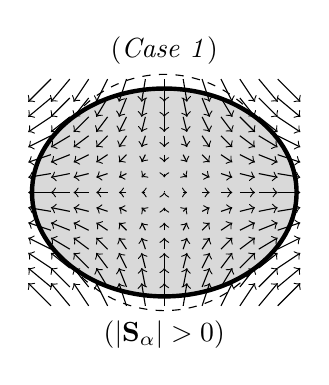
\begin{tikzpicture}[ultra thick,scale=0.6]
        \def\nRows{6}
        \def\nCols{6}
        \draw[dashed,thin] (0,0)circle(2.5);
        \draw[fill=gray!30] (0,0)ellipse(2.8 and 2.2);
        \foreach \x in {-\nRows,...,\nRows} {
            \foreach \y in {-\nCols,...,\nCols} {
                \pgfmathsetmacro\distance{veclen(\x*0.4, \y*0.4)};
                \pgfmathparse{\distance < 2.45 ? "blue" : "white"}
                \edef\colour{\pgfmathresult};
                \ifthenelse{\equal{\colour}{blue}}{                    
                    \draw[thin,->](\x*0.4,\y*0.4)--++(0.08*\x,-0.08*\y);
                }
            }
        }
        \node (txt) at (0,3){(\textit{Case 1})};
        \node (txt) at (0,-3){($|\textbf{S}_\alpha| > 0$)};
    \end{tikzpicture}
     \hfill
    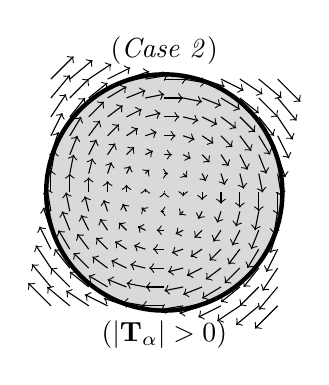
\begin{tikzpicture}[ultra thick,scale=0.6]
        \def\nRows{6}
        \def\nCols{6}
        \draw[fill=gray!30] (0,0)circle(2.5);
        \foreach \x in {-\nRows,...,\nRows} {
            \foreach \y in {-\nCols,...,\nCols} {
                \pgfmathsetmacro\distance{veclen(\x*0.4, \y*0.4)};
                \pgfmathparse{\distance < 2.5 ? "blue" : "white"}
                \edef\colour{\pgfmathresult};
                \ifthenelse{\equal{\colour}{blue}}{                    
                    \draw[thin,->](\x*0.4,\y*0.4)--++(0.08*\y,-0.08*\x);
                }
            }
        }
        \node (txt) at (0,3){(\textit{Case 2})};
        \node (txt) at (0,-3){($|\textbf{T}_\alpha| > 0$)};
    \end{tikzpicture}
    \hfill
    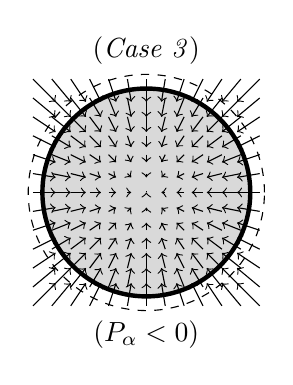
\begin{tikzpicture}[ultra thick,scale=0.6]
        \def\nRows{6}
        \def\nCols{6}
        \draw[dashed,thin] (0,0)circle(2.5);
        \draw[fill=gray!30] (0,0)circle(2.2);
        \foreach \x in {-\nRows,...,\nRows} {
            \foreach \y in {-\nCols,...,\nCols} {
                \pgfmathsetmacro\distance{veclen(\x*0.4, \y*0.4)};
                \pgfmathparse{\distance < 2.3 ? "blue" : "white"}
                \edef\colour{\pgfmathresult};
                \ifthenelse{\equal{\colour}{blue}}{                    
                    \draw[thin,->](\x*0.4,\y*0.4)--++(-0.08*\x,-0.08*\y);
                }
            }
        }
        \node (txt) at (0,3){(\textit{Case 3})};
        \node (txt) at (0,-3){($P_\alpha < 0$)};
    \end{tikzpicture}
    \hfill
    \caption{Graphical representation of the inner kinematics   of an arbitrary particle under three scenarios. 
        The arrows represent the velocity field inside the particle, $\textbf{w}_d^0$, with the corresponding value of the moment of momentum tensor indicated below. 
        The operator $|\ldots|$ refers to the norm of the tensors. 
        According to the inner velocity field:
        (\textit{Case 1}) The particle experiences a mean deformation, resulting in non-zero stretching of momentum along the principal axis of deformation;
        (\textit{Case 2}) The particle is rotating, leading to a non-zero angular momentum vector in the direction of rotation;
        (\textit{Case 3}) The particle undergoes compression, resulting in a negative trace of the moment of momentum.
    }
    \label{eq:scheme}
\end{figure}
Injecting, $f_d^0 = \rho_d$ in the second-order moment equation (derived in \ref{ap:Moments_equations}) we obtain,
%\JL{pq lequation du second moment de la masse ne fait pas intervenir la trace du premier moment de la qdm - cela semble incoherent ?}
\begin{equation}
    \ddt {\textbf{M}_\alpha}=2(\textbf{S}_\alpha+P_\alpha\bm\delta),
    \label{eq:dt_M_alpha}
\end{equation}
which is the second-order moment of mass conservation equation assuming that the fluid within the drop is divergence free. 
From \ref{eq:dt_M_alpha} we deduce that the evolution of the distribution of mass of a particle is solely determined by the  of momentum $\textbf{S}_\alpha$ and $P_\alpha$. 
This indicates that angular momentum does not influence the evolution of the second moment of mass, a consequence of the symmetry of the tensor $\textbf{M}_\alpha$, which must be preserved after differentiation with respect to time.
However, this does not imply that the particle angular velocity ($\bm\omega_\alpha$) does not appear in this equation. 
For instance, in the case of rigid body motion where $\textbf{w}_d^0 = \bm\omega_\alpha \times \textbf{r}$, we obtain the relation  $2(\textbf{S}_\alpha)_{ij} = \epsilon_{iab} (\bm\omega_\alpha)_a (\textbf{M}_\alpha)_{bj}+ 
\epsilon_{jab} (\bm\omega_\alpha)_a (\textbf{M}_\alpha)_{bi}  $. 

Now that we have described the kinematics   of the particle shape, let us proceed to derive an equation for the moment of momentum.
This equation is derived by injecting $\textbf{Q}_\alpha^{(1)} = \textbf{P}_\alpha$ in \ref{eq:dt_Q_alpha_tot}, it reads, 
\begin{equation}
    \ddt {\textbf{P}_\alpha}
    - \intO{ \rho_d  \textbf{w}_d^0 \textbf{w}_d^0 }
    = 
    - \intO{\bm{\sigma}_d^0}
    - \intS{ 
        \gamma (\bm\delta - \textbf{nn})
    }
    + \intS{ \textbf{r}\bm{\sigma}_f^0\cdot \textbf{n}}.
    \label{eq:dt_P_alpha}
\end{equation}
In the following sections the normal vector noted \textbf{n} always refer to $\textbf{n}_d$. 
The conservation equation of the angular momentum $\bm{\mu}_\alpha$ is obtained by taking the double contracted product of \ref{eq:dt_P_alpha} with $\bm\epsilon$, which directly gives
\begin{equation}
    \ddt\bm{\mu}_\alpha
    =  
    % \textbf{t}_\alpha.
    \intS{ \textbf{r} \times \bm{\sigma}_f^0\cdot \textbf{n} }
    \label{eq:dt_mu_alpha}
\end{equation}
Note that every term on the right-hand side of \ref{eq:dt_P_alpha} vanished due to their symmetric nature apart from the skew-symmetric part of the hydrodynamic stress, which is the hydrodynamic torque applied on the particle $\alpha$.
In particular, the surface tension terms do not appear in the angular momentum balance since the tensor $\bm\delta-\textbf{nn}$ is symmetric, which is consistent with the findings of \citet{hesla1993note}. 
As a consequence, the surface tension does not affect the angular momentum regardless of the particle shape. 
%In the literature, it is common to include the torque due to inter-particular interactions in the angular momentum balance, as is done in \citet{jackson1997locally} and \citet{zhang1997momentum}.
%In our case note that $\bm{\sigma}_f^0$ contains short-range hydrodynamic interaction forces. 

Taking the symmetric part of \ref{eq:dt_P_alpha}, and substrating the trace yields, 
\begin{align}
    &\ddt {\textbf{S}_\alpha}
    - \rho_d\intO{\left(\textbf{w}_d^0 \textbf{w}_d^0 -\frac{1}{3} (\textbf{w}_d^0 \cdot  \textbf{w}_d^0)\bm\delta\right)}
    = \nonumber \\
    &- 2\mu_d\intO{\textbf{e}_d^0}
    -  \intS{ \gamma
        \left( \frac{1}{3}\bm\delta - \textbf{nn} \right)
    }
    + \frac{1}{2}\intS{\left(\textbf{r}\bm\sigma_f^0+\bm\sigma_f^0\textbf{r}-\frac{2}{3}(\bm\sigma_f^0 \cdot \textbf{r})\bm\delta \right)\cdot \textbf{n}},
    \label{eq:dt_S_alpha}
\end{align}
%internal velocity kinetic energy. %$\intO{\rho_d\textbf{w}_d^0\textbf{w}_d^0 }$.
%On the left-hand side of \ref{eq:dt_S_alpha} we identify two inertial terms, i.e. the derivative of $\textbf{S}_\alpha$ and the stress induced by the product of internal velocity within the drop.
%The inertia of the particle is then balanced by the terms on the right-hand side of the equation, namely: 
%the volumic integral of the particle viscous stress; 
%the surface integral of the surface tension stress ; 
%and the first moment of the hydrodynamic stress tensor.
%A discussion regarding the physical implications of this equation is provided below. 
where we have introduced the rate of strain tensor for phase \( k \), defined as \( \mathbf{e}_k^0 = \frac{1}{2} (\grad \mathbf{u}_k^0 + ^\dagger \grad \mathbf{u}_k^0) \). 
Here $^\dagger$ represents the transpose operator. 
On the left-hand side of \ref{eq:dt_S_alpha}, two inertial contributions can be identified: the time derivative of $\mathbf{S}_\alpha$, and the stress arising from the product of internal velocity field within the droplet. 
These inertial effects are counterbalanced by the terms appearing on the right-hand side of the equation, which include: the volume integral of the particle viscous stress; the surface tension moment; and the first moment of the hydrodynamic force.
%\JL{a finaliser}
While surface tension effects do not influence the linear or angular momentum equations directly, they do impact the moment of momentum $\textbf{P}_\alpha$, specifically its symmetric part $\textbf{S}_\alpha$.
Consequently, surface tension influences the hydrodynamic behavior of a particle exclusively through its effect on $\textbf{S}_\alpha$, which is related to the shape of a particle represented by $\textbf{M}_\alpha$, via \ref{eq:dt_M_alpha}.
%Whether it is solid or fluid particles \ref{eq:dt_S_alpha} becomes particularly relevant for expressing the averaged stress within an inertial suspension in terms of Lagrangian properties, as discussed in the next chapter. 
%\JL{enlever la trace}
%Taking the symmetric part of \ref{eq:dt_P_alpha}, and making use of \ref{eq:dt_M_alpha}, yields a dynamical balance equation for $\textbf{M}_\alpha$, namely
Inserting \ref{eq:dt_S_alpha} in  \ref{eq:dt_M_alpha} yields,
%\JL{enlever la trace et reecrire la partie ci-dessous + donner la definition de $e_d$ qui n'est pas de defini avant.}
\begin{align}    
    &\frac{1}{2}\frac{d^2 (\textbf{M}_\alpha-\frac{1}{3}(\textbf{M}:\bm\delta)\bm\delta)}{dt^2}
    =  \rho_d\intO{\left(\textbf{w}_d^0 \textbf{w}_d^0 -\frac{1}{3} (\textbf{w}_d^0 \cdot  \textbf{w}_d^0)\right)}
    - 2\mu_d\intO{\textbf{e}_d^0} \nonumber\\
    &- \intS{\gamma  
        \left( \frac{1}{3}\bm\delta - \textbf{nn} \right)
    }
    + \frac{1}{2}\intS{\left(\textbf{r}\bm\sigma_f^0+\bm\sigma_f^0\textbf{r}-\frac{2}{3}(\bm\sigma_f^0 \cdot \textbf{r})\bm\delta \right)\cdot \textbf{n}}.
    \label{eq:dt2_M_alpha}
\end{align}
%On the left-hand side of \ref{eq:dt_S_alpha}, we recover the symmetric part of the inertial contributions. 
%In opposition to \ref{eq:dt_P_alpha} we could substitute the term $\ddt (\textbf{P}_\alpha+\textbf{P}_\alpha^\dagger)$ initially present in the equation by $\ddt^2 \textbf{M}_\alpha$ using \ref{eq:dt_M_alpha}. 
%\ref{eq:dt2_M_alpha} is a second-order partial differential equation for the second order mass moment characterizing the droplet shape.
%In other words, \ref{eq:dt2_M_alpha} must be interpreted as an equation for the shape of the particle, represented by the tensor $\textbf{M}_\alpha$. 
%Thus, on the right-hand side of \ref{eq:dt_S_alpha}, we identify the terms which favors deformation, including the inertia of the velocity field within the droplet as well as the traceless part of the first moment and the terms wwohc resis deformation incluidng the viscous resistance within the droplet and the surface tension.
\ref{eq:dt2_M_alpha} is a second-order differential equation governing the second-order mass moment that characterizes the droplet shape. 
In other words, it should be interpreted as an equation describing the droplet shape, represented by the traceless part of the tensor $\textbf{M}_\alpha$.
Accordingly, the right-hand side of \ref{eq:dt2_M_alpha} contains terms that promote deformation-such as the product of the internal velocity field and the traceless component of the first moment as well as terms that oppose deformation, including droplet internal viscous resistance and surface tension.
%One might also recognize that \ref{eq:dt2_M_alpha} is in fact an extension of \citet{batchelor1970stress} result, but with the consideration of the inertia of the particle.
\ref{eq:dt2_M_alpha} is particularly useful to compute the unknown internal stress within solid particles, in terms of surface integral, i.e. the first moment of the hydrodynamic force.
This relation plays a key role in expressing the bulk stress of a suspension and ultimately leads to the effective viscosity, once a closed-form expression for the average first moment is obtained \citep{batchelor1970stress}. 
In the inertial regime, and for solid particles, the tensors $\textbf{M}_\alpha$ and the internal velocity field $\textbf{w}_d^0$ are fully prescribed by the particle kinematics. 
As a result, in \ref{eq:dt2_M_alpha}, $\textbf{M}_\alpha$ and $\textbf{w}_d^0$ appear not as unknowns but rather as known source terms.
For spherical particles specifically, the inertial correction to the first force moment has been derived by \citet{hwang1989modeling} and  \citet{lhuillier1996contribution}.
%For the specific case of spherical particles \citet{hwang1989,lhuillier1996contribution} have derived this inertial correction.
%This relation is used to express the bulk stress of a suspension.
%It eventually leads to the computation of the famous Einstein equivalent viscosity, upon having a closed expression for the average of the first moment \citep{guazzelli2011}. 
%In the inertial case and for solid particle, the tensors $\textbf{M}_\alpha$ and the inner velocity field $\textbf{w}_d^0$ are fully determined by the particle kinematic, indicating that $\textbf{M}_\alpha$ and $\textbf{w}_d^0$ can be used in \ref{eq:dt_S_alpha} not as unknowns but as source terms. 
%Consequently, for solid particles, \ref{eq:dt_S_alpha} must be interpreted as a generalized equation for the undefined stress $\bm\sigma_d^0$ integrated on the volume of the particles.

%Note that if intead we had considered spherical particles composed of compressible fluid \ref{eq:dt2_M_alpha} transforms into the Rayleigh-Lamb-Plesset equation as demonstrated in \citep{danielcours}.


%In our case, only the external contribution $\intS{\textbf{r}\bm\sigma_f^0\cdot \textbf{n}}$ is responsible for the generation of angular momentum, see \ref{eq:dt_mu_alpha}.
%Taking the symmetric part of this tensor ultimately removes this contribution. 

%\begin{equation}
%    \intO{\bm{\sigma}_d^0}
%    + \intS{\gamma(\bm\delta - \textbf{nn})}
%    = \frac{1}{2}\intS{(\textbf{r}\bm\sigma_f^0+\bm\sigma_f^0\textbf{r})\cdot \textbf{n}},
%    \label{eq:Batchelor}
%\end{equation}

%In \ref{ap:Moments_equations} we show how to derive the higher-order moment of momentum equations, which can also be viewed as formulas for the higher moments of the internal particle stress distribution. 
%It is interesting to mention that in a recent study of \citet{dolata2021faxen} and \citet{zhou2020lamb} they make use of the first two moments of momentum equations hidden into another but equivalent form, valid in the Stokes flow regime. 








\subsection{Averaged momentum and mass conservation equations}



Let us now focus on the averaged momentum equation of the continuous phase. 
By applying \eqref{eq:dt_f_k} with $f_k = \rho_f$ and $\rho_f\textbf{u}_f$ we obtain the mass and momentum equation for the continuous phase under the two fluid formulation, 
\begin{align}
    (\pddt + \textbf{u}_f\cdot \grad)\textbf{u}_f&=-\phi_f \div \textbf{u}_f
    \label{eq:mass_init}\\
    \phi_f \rho_f(\pddt + \textbf{u}_f  \cdot \grad) \textbf{u}_f
    % +  \div \avg{\chi_f\rho_f \textbf{u}_f'\textbf{u}_f'}
    &= 
    \div [\phi_f \bm\sigma_f-  \avg{\chi_f\rho_f \textbf{u}_f'\textbf{u}_f'}]
    + \phi_f \rho_f \textbf{g}
    - \avg{\delta_\Gamma \bm\sigma_f\cdot \textbf{n}}.
    \label{eq:two_fluid_momentum_init}
\end{align} 
To obtain the hybrid formulation one can expand the final term on the right-hand side of \ref{eq:two_fluid_momentum_init} using the Taylor expansion provided in \ref{eq:f_exp}.  
However, before doing so, it is important to examine the term \( \phi_f \bm\sigma_f \), as it contains a non-closed contribution originating from the averaging of the strain rate tensor. %a contribution from the dispersed phase. 
Properly identifying and isolating this contribution is a necessary step prior to performing the Taylor expansion.
%Moreover, there

%one may use \ref{eq:f_exp} to taylor expand the last term on the right-hand side of \ref{eq:two_fluid_momentum_init}. 
%However, it is first important to discuss the form of the term $\phi_f\bm\sigma_f$ since a dispersed phase term, is hidden into it, hence it is important to identify this term before carrying out the Taylor expansion. 

%\subsection{Mean stress formulation and momentum transfer decomposition}
%\JL{bien expliquer quand et comment apparaissent les distinctions sur le choix de la contrainte moyenne. en particulier voir en dessous}

We begin by noting that $\phi_f\bm\sigma_f$ can be expressed in terms of the averaged fluid pressure $p_f$, and continuous phase averaged velocity ($\textbf{u}_f$), or bulk-averaged velocity ($\textbf{u} = \phi_f \textbf{u}_f + \phi_d \textbf{u}_d$).
Expressing $\bm\sigma_f$ as a function of $\textbf{u}_f$ instead of $\textbf{u}$ (or vice versa) leads to two distinct forms of the momentum equation, each associated with different formulations of the closure terms. 
We also review several alternative choices found in the literature (see also \citet{jackson2000, pahtz2025general} for an overview focused on solid particles), emphasizing that while all these formulations are mathematically equivalent, they give rise to different closure problems. 
We argue that one particular formulation is probably the most suitable, especially in light of the closure terms available in the literature for non-dilute flows.%especially in the context of existing closure models for non-dilute flows.
%Choosing to express $\bm\sigma_f$ as a function $\textbf{u}_f$ rather than $\textbf{u}$ and vice versa, results in two distinct forms of the momentum equation and two distinct formulations of the closure terms. 
%We also discuss the various other choice available on the literature (see also \citet{jackson2000,pathz2025} for a review for solid particles) explaining that there is all choice are perfectly equivalent but leads to a different closure problems.
%Our belief his that there is one formulation which is the most appropriate with respect to of the closure terms available in the litterature for non-dilute flow.
%Although this topic has been already discussed in the context of solid particles  we propose here to expose both formulations and discuss which of the two equivalent (but different) formulations is the most suited for multiphase flow modeling. 

%Because we believe this topic has not been discussed much for non-solid particles in the literature, we propose here to expose both formulations and discuss which of the two equivalent (but different) formulation is the most suited for multiphase flow modeling. 
%Because we believe this topic has not been discussed much in the literature for non-solid particles, 

First we introduce what we refer to as the \textit{mean Newtonian stress}, based either on the continuous phase averaged velocity $\textbf{u}_f$ or on the bulk velocity \textbf{u}, namely,
\begin{align}
    \bm\Sigma_f 
    &
    = -p_f \bm\delta + 2\mu_f \textbf{E}_f    
    %= -p_f \bm\delta + \mu_f [\grad \textbf{u}_f + (\grad \textbf{u}_f)^{\dagger}], 
    \label{eq:Sigma_f_average}
    \\
    \bm\Sigma &
    = -p_f\bm\delta + 2 \mu_f \textbf{E}
    %= -p_f \bm\delta + \mu_f [\grad \textbf{u} + (\grad \textbf{u})^{\dagger}],
    \label{eq:Sigma_average}
\end{align}
where $\textbf{E}_f = [\grad \textbf{u}_f + (\grad \textbf{u}_f)^{\dagger}]/2$ and $\textbf{E} =[\grad \textbf{u} + (\grad \textbf{u})^{\dagger}]/2$ represent the \textit{mean strain rate} tensor based either on $\textbf{u}_f$ or on \textbf{u}. 
Additionally the ensemble averaged stress $\phi_f \bm\sigma_f$ may be written as 
\begin{equation}
    \phi_f \bm\sigma_f = - \phi _f p_f \bm\delta + 2 \mu_ f \phi_f \textbf{e}_f
    \label{eq:sigma_average}
\end{equation}
where $\phi _f \textbf{e}_f = \avg{\chi _f \textbf{e}_f^0}$. 
%Moreover by definition the bulk stress tensor reads $\textbf{E} = \phi _f\textbf{e}_f + \phi_d \textbf{e}_d$.
Inserting \ref{eq:Sigma_f_average} and \ref{eq:Sigma_average} in  \ref{eq:sigma_average} yields
%Using the constitutive law of Newtonian fluids we find, 
\begin{align}
    \phi_f \bm\sigma_f 
    &=
    % - \phi_f p_f \bm\delta
    % + \phi_f \mu_f [\grad \textbf{u}_f  + (\grad \textbf{u}_f)^\dagger]
    % - \mu_f \avg{\delta_\Gamma( \textbf{u}_f'  \textbf{n} +  \textbf{n} \textbf{u}_f' )}
    % =
    \phi_f \bm\Sigma_f
    - \mu_f \avg{\delta_\Gamma( \textbf{u}_f'  \textbf{n} +  \textbf{n} \textbf{u}_f' )}
    \label{eq:stress_closure}\\
    \phi_f \bm\sigma_f 
    &=
    % - \phi_f p_f \bm\delta
    % + \mu_f [\grad \textbf{u}  + (\grad \textbf{u})^\dagger]
    % - 2\mu_f \phi_d \textbf{e}_d
    % =
    \phi_f \bm\Sigma
    - \avg{2\mu_f \chi_d \textbf{e}_d^*}
    \label{eq:stress_closure1}
\end{align}
where we have used the relations 
\begin{equation}
    \avg{\chi_f \grad \textbf{u}_f^0}
    = 
    \phi_f \grad  \textbf{u}_f
    + \avg{\delta_\Gamma \textbf{n}_f \textbf{u}_f'}
    \label{eq:first_rel}
\end{equation}
and
\begin{equation}
    %\avg{\chi_f \textbf{e}_f^0}
%    = 
%    \avg{\textbf{e}^0}
%    - \avg{\chi_d \textbf{e}_d^0}
\phi _f\textbf{e}_f
%    = 
%    \textbf{E}
%    - \avg{\chi_d \textbf{e}_d^0}
    = 
    \phi_f \textbf{E}
    - \avg{\chi_d \textbf{e}_d^*},
    \label{eq:sec_rel}
\end{equation}
to derive \ref{eq:stress_closure,eq:stress_closure1}, respectively. 
 %in most practical situations of interest.
%Note that \ref{eq:first_rel} remains true in the presence of non zero interfacial rate of strain, while \ref{eq:sec_rel} requires the condition that the bulk rate of strain reads $\textbf{E} = \phi _f\textbf{e}_f + \phi_d \textbf{e}_d$ \textit{i.e.} that there is no shear stress at the interface of the droplets, so that $\avg{\delta_\Gamma \textbf{e}_\Gamma^0}= 0$, which is true in most of the practical cases of interest. 
In \ref{eq:stress_closure1} we have introduced $\textbf{e}_d^* = \textbf{e}_d^0 - \textbf{E} = \grad (\textbf{u}_d^0-\textbf{u})+\grad (\textbf{u}_d^0-\textbf{u})^\dagger$ which is the droplet internal shear rate relative to the `bulk' shear rate \textbf{E}.
%While $\textbf{u}_f' = \textbf{u}_f^0 - \textbf{u}_f$ in \ref{eq:stress_closure}. 
It is worth noting that \ref{eq:first_rel} remains valid even when the interfacial rate of strain is nonzero. 
In contrast, \ref{eq:sec_rel} holds under the assumption that the bulk rate of strain satisfies $\textbf{E} = \phi_f \textbf{e}_f + \phi_d \textbf{e}_d$, \textit{i.e.} that $\avg{\delta_\Gamma \textbf{e}_\Gamma^0} = 0$. 
This condition is supposed to be met here because we did not consider interfacial viscosity\citep{nadim1996concise}.
%Before presenting the hybrid form of the continuous phase momentum equation, it is interesting to expose the classic two-fluid formulation using the stress formulation given by \ref{eq:stress_closure} in the first place. 
%Before introducing the hybrid form of the continuous phase momentum equation, it is useful to first present the classical two-fluid formulation, employing the stress formulation \ref{eq:stress_closure}.
The averaged momentum equation  employing the stress formulation \ref{eq:stress_closure} read, 
\begin{align}
    % (\pddt + \textbf{u}_f\cdot \grad)\textbf{u}_f&=-\phi_f \div \textbf{u}_f\\
    \phi_f \rho_f(\pddt + \textbf{u}_f  \cdot \grad) \textbf{u}_f
    % +  \div \avg{\chi_f\rho_f \textbf{u}_f'\textbf{u}_f'}
    &= \phi_f 
    \left(\div \bm{\Sigma}_f
    + \rho_f \textbf{g}\right)
    - \div 
    [\avg{\chi_f\rho_f \textbf{u}_f'\textbf{u}_f'}
    +\avg{\delta_\Gamma \mu_f( \textbf{u}_f'  \textbf{n} +  \textbf{n} \textbf{u}_f')}]
    - \avg{\delta_\Gamma \bm\sigma_f^{(1)}\cdot \textbf{n}},
    \label{eq:two_fluid_momentum}
\end{align}
where, $\bm\sigma_f^{(1)}=\bm\sigma_f^0 - \bm\Sigma_f$ which also reads %is the Newtonian stress evaluated at a point on an interface relative to the mean stress $\bm\Sigma_f$. 
\begin{equation}
\bm\sigma_f^{(1)} = -p_f'\bm\delta
+ \mu_f [
    \grad \textbf{u}_f'
    + ^\dagger \grad \textbf{u}_f']
    \label{eq:disturbance_stress1}
\end{equation} 
Likewise, using \ref{eq:stress_closure1} one may also derive another form of the momentum equation, namely,
\begin{equation}
    \phi_f \rho_f(\pddt + \textbf{u}_f  \cdot \grad) \textbf{u}_f
    % +  \div \avg{\chi_f\rho_f \textbf{u}_f'\textbf{u}_f'}
    = \phi_f 
    \left(\div \bm{\Sigma}
    + \rho_f \textbf{g}\right)
    - \div 
    [\avg{\chi_f\rho_f \textbf{u}_f'\textbf{u}_f'} + \avg{2\mu_f \chi_d \textbf{e}_d^*}]
    - \avg{\delta_\Gamma \bm\sigma_f^{(2)}\cdot \textbf{n}},
    \label{eq:two_fluid_momentum2}
\end{equation} 
where $\bm\sigma_f^{(2)}=\bm\sigma_f^0 - \bm\Sigma$. 
%This stress tensor corresponds to the Newtonian stress (relative to the mean pressure and velocity field) typically available in numerical or theoretical studies. 
It can be also expressed as, 
%Clearly, subtracting by $\bm\Sigma_f$ to the local stress at the interface leads to the expression 
\begin{equation}
    \bm\sigma_f^{(2)} 
    =
    -p_f'\bm\delta
    + \mu_f [
        \grad \textbf{u}_f^*
        + ^\dagger \grad \textbf{u}_f^*
    ]
    \label{eq:disturbance_stress2}
\end{equation}
where $\textbf{u}_f^*= \textbf{u}_f^0 - \textbf{u}$.
%which corresponds to the Newtonian stress at the surface of the droplets (relative to the mean pressure and velocity field) typically available in numerical or theoretical studies.
%Likewise, substituting the mean stress with $\bm\Sigma$ in \ref{eq:disturbance_stress} one obtain the same formula except than $\textbf{u}_f'\to \textbf{u}_f^0 - \textbf{u}$. 
%Hence, 
In both cases (\ref{eq:two_fluid_momentum} and \ref{eq:two_fluid_momentum2}) one has to compute the local stress relative to the averaged continuous phase motion or bulk phase motion. 
% Note that because $\div \textbf{u} = 0$ it may be more convenient to  
%Note the differences between the last term of formulation \ref{eq:stress_closure} and \ref{eq:stress_closure1}, is equal to, $\phi_f (\div \bm\Sigma_f - \div\bm\Sigma)$
%Hence, the transition from one formulation to the other is straightforward, it just requires adding or subtracting $\phi_f (\div \bm\Sigma_f - \div\bm\Sigma)$. 
%However it is worth noting the physicsical meaning og this term which also reads,
Note the difference between the last terms in formulations \ref{eq:stress_closure} and \ref{eq:stress_closure1}, which is given by $\phi_f \div (\bm\Sigma_f -\bm\Sigma)$.
The transition from one formulation to the other is straightforward and only requires the addition or subtraction of this term. 
However, it is important to recognize its physical significance.
This difference can be expressed explicitly as,
\begin{equation}
    \phi_f \div(\bm\Sigma_f - \bm\Sigma) = \mu_f \phi_f \div \left[\grad (\phi_d (\textbf{u}_f - \textbf{u}_d)) + \grad (\phi_d (\textbf{u}_f - \textbf{u}_d))^\dagger \right]
    \label{eq:diff_sigma1}
\end{equation}
where the decomposition 
\begin{equation}
\textbf{u} = \phi_f \textbf{u}_f + \phi_d \textbf{u}_d,
\label{eq:u_mean} 
\end{equation}
has been used in the derivation.
\ref{eq:diff_sigma1} reveals that the difference between the two formulations introduces a non-Newtonian stress term.
This non-Newtonian stress shares similarities with the second-order force moment closure \citep{jackson1997locally,zhang1997momentum}, and it is typically related to intrinsic convection in sedimentation processes \citep{lhuillier2022}.
Therefore, when addressing the closure problem, it is essential to treat each stress formulation carefully, as the inclusion or exclusion of this additional term can significantly impact the resulting model.
%Then, when considering the colsure problem one has to be carefull to properly consider each formulation of the stress differently as both formulation will resulst in adding or removing this term.
%between \ref{eq:def_sigma_eff_f} and \ref{eq:def_sigma_eff_f2}  plus the differences between the corresponding drag force terms, is exactly equal to, $\phi_f (\div \bm\Sigma_f - \div\bm\Sigma)$.
%\JL{il faut que tu m'expliques : quand je soustrais les forces j'obtiens $\phi (\div \bm\Sigma_f - \div\bm\Sigma)$. OK on soustrait juste le RHS par ailleurs je pense qu'il faut detailler cela, c'est un point important.}
%\JL{en particulier $\div \bm\Sigma_f - \div\bm\Sigma = \div \nabla u_f - u \propto u_r$  a expliciter en montrant le developpment limite}





%Even though, both stress decomposition and momentum formulations proposed here are equivalent, each formulation have advantages and drawback which we discuss below.  
Although the stress decomposition and momentum formulations proposed herein are mathematically equivalent, each presents distinct advantages and limitations, which we examine in detail below.
%Now let us discuss on the choic between $\bm\Sigma$ and $\bm\Sigma_f$. 
%At first sight, using \ref{eq:dt_uf} with the effective stress given by \ref{eq:def_sigma_eff_f}, seems more practical because we are solving for the field $\textbf{u}_f$ hence avoiding the need of \ref{eq:velocity_conservation}. 
First, we may observe that a simplification arises for \ref{eq:stress_closure1} in the case of solid particles, for which $\textbf{e}_d^0 = 0$.
As a result $\phi _f \bm \sigma _f = - \phi _f p_f \bm\delta + 2 \mu_ f \textbf{E}$ \citep{joseph1990ensemble,jackson2000}. %and $\avg{\chi_d \textbf{e}_d^*} = -\phi\bm\Sigma$. \JL{a montrer}
Owing to this simplification, the formulation based on $\bm\Sigma$ and the associated closure relation \eqref{eq:stress_closure1} makes it a good candidate to be used in practice for solid particles. %is frequently adopted in the literature \citep{jackson2000}, despite requiring the inclusion of the additional momentum conservation equation.
Second, employing \ref{eq:two_fluid_momentum} with \ref{eq:disturbance_stress1} may appear more convenient as the governing equations are directly formulated in terms of the fluid velocity field $\textbf{u}_f$, thereby circumventing the need to explicitly include an expansion for the bulk fluid velocity. %the following equation
%Because $\textbf{u}$ may be required by \ref{eq:stress_closure1}, one also need to solve the equation, 
%\eqref{eq:velocity_conservation}.
%On the other hand we note that for solid particles $\textbf{e}_d^0 = 0$ and $\avg{\chi_d \textbf{e}_d'} = -\bm\Sigma\phi$, because of this great simplification \ref{eq:stress_closure1} is often used \citep{jackson2000} even if it requires adding \ref{eq:velocity_conservation} in the system of equation.  
%\JL{Je comprends l'interet de cette simplification, mais il faur toujours avoir une exression pr $\textbf{E}$ donc pour $\textbf{u}$}
Third, there exists a conceptual reason for preferring the bulk stress $\bm\Sigma$ when deriving closure relations for non-dilute suspensions.  %involving the fluctuating stress $\bm\sigma_f'$. 
Specifically, because $\bm\sigma_f^{(2)}$ depends on the disturbance velocity $\textbf{u}_f^* = \textbf{u}_f^0 - \textbf{u}$, the averaged velocity $\textbf{u}$ naturally serves as the "far-field" or "undisturbed" velocity boundary condition in the conditionally averaged Navier-Stokes equations \citep{hinch1977averaged,fintzi2025}. %(as also emphasized in the context of this PhD study).
%But there is another reason for using the `bulk stress' $\bm\Sigma$ as a reference stress to compute the closure terms involving $\bm\sigma_f'$. 
%Indeed, since $\bm\sigma_f'$ requires $\textbf{u}_f' = \textbf{u}_f^0 - \textbf{u}$, then \textbf{u} becomes the `far field' or `undisturbed' velocity boundary condition far from the test particle in the conditionally averaged Navier-Stokes equations \tb{(+my phd)}.
%On another hand, one may note that all the available theoretical solutions considering the disturbance field of a particle embedded in a pure solvent or in an effective medium (which represents other particles' contribution) use a divergence free `background flow' as limiting condition \citep{kim1985modelling,hinch1977averaged}.
%Since $\div \textbf{u} =0$ we deduce that the velocity field used in most (if not all) theoretical problems correspond to \textbf{u}. 
%Therefore, the disturbance  stress computed in these problems is $\bm\sigma_f'= \bm\sigma_f^0 - \bm\Sigma$. 
Notably, most (if not all) existing theoretical solutions addressing the disturbance field generated by a particle embedded in a Newtonian solvent or in an effective medium - representing other particles contribution - use a divergence-free background velocity field as limiting boundary condition \citep{hinch1977averaged, kim1985modelling}. 
Since $\div \textbf{u} = 0$, it follows that the velocity field used in these theoretical study corresponds to $\textbf{u}$. 
Consequently, the disturbance stress derived in those studies is $\bm\sigma_f^{(2)} = \bm\sigma_f^0 - \bm\Sigma$.
In opposition, the stress decomposition based on $\bm\Sigma_f$, involves the fields $\textbf{u}_f$ which is not divergence free. 
Hence, this `far field' or `undisturbed' velocity boundary condition far from the test particle does not correspond to the usual boundary condition assumed in most of the theoretical problems. 
%In conclusion, it is important to note that \textbf{u} corresponds exactly to the `background velocity' fields used in most of the theoretical derivations.
%Hence, the resulting closure terms (drag forces, stresslet and higher moments) derived in these studies refer to the closures expressed in terms of $\bm\sigma_f^0 - \bm\Sigma$.
%In all case one can always express $\bm\Sigma_f$ in terms of $\bm\Sigma$ hence which formulation to use is not a fatality. 
%However, one must always be careful when asserting that a given formulation of the drag force, for example, is exactly equivalent to a closure term found in the literature, as there are multiple possible formulations  (either based on $\bm\Sigma_f$, $\bm\Sigma$, $\bm\sigma_f$ or even  $p_f \bm\delta$). 
%Note that the choices between $\bm\Sigma_f$ and $\bm\Sigma$ only matter if one consider a closure problem, in which $\phi \textbf{u}_f \neq \phi \textbf{u}$, hence accurate at $O(\phi^2)$ at least (such as in \citet{hinch1977averaged,kim1985modelling}). 
In conclusion, it is important to recognize that the vector field \(\textbf{u}\) corresponds precisely to the 'background velocity' typically employed in theoretical derivations. 
Consequently, the closure terms obtained in such analyses -such as the hydrodynamic forces, the stresslet, and higher-order moments- are formulated in terms of the difference \(\bm\sigma_f^0 - \bm\Sigma\).
Of course, it is always possible to express \(\bm\Sigma_f\) in terms of \(\bm\Sigma\) (see \ref{eq:diff_sigma1}), meaning that the choice of formulation remains free. 
Nevertheless, we must be cautious when claiming that a specific expression of, for example, the Faxen contribution to the force is exactly equivalent to a closure term reported in the literature especially for non-dilute suspension. 
%Multiple valid formulations exist, involving \(\bm\Sigma_f\), \(\bm\Sigma\), \(\bm\sigma_f\), or even the pressure tensor \(p_f \bm\delta\).
% It should also be noted that the distinction between $\bm\sigma_f^{(1)}$ and $\bm\sigma_f^{(2)}$ becomes relevant only in the context of closure problems accurate at \(O(\phi^2)\) or more\footnote{Indeed, because $\textbf{u} \phi = \textbf{u}_f\phi +O(\phi^2)$ the distinction between bulk or continuous phase averaged velocity field becomes irrelevant in the closure problem. }. 
% \JL{pas compris cette derniere phrase que je pense il faut enlever : on montre que la distinction joue deja pour le second moment des forces en regime dilue non ?}

% \JL{je n'ai pas compris le paragraphe suivant - je ne sais pas si il est necessaire desormais vu l'organisation actuelle ou on fait le developement en serie de Taylor plus tard}
% One can remark the similarities between the surface exchange terms expansion, and the multipole expansion used in microhydrodynamic that characterize the disturbance field caused by a body immersed in a stokes flow \citet{pozrikidis1992boundary,kim2013microhydrodynamics}. 
% Moreover, one can wonder which of the formulation, \ref{eq:def_sigma_eff_f2} or \ref{eq:def_sigma_eff_f}, contains what is called the `Stresslet' and the higher moments of force given by the multipole expansion used in microhydrodynamic ? \citep{pozrikidis1992boundary,kim2013microhydrodynamics}\footnote{Note that the first term in this expansion is the same whether we use \ref{eq:def_sigma_eff_f2} or \ref{eq:def_sigma_eff_f}}.   
% These moments are usually defined as the `extra stress above the value of the fluid law'\citep{hinch1977averaged}.
% Because we are not studying the `bulk' momentum equation this definition does not directly apply in our context. 
% However, note that \ref{eq:stress_closure1} involves the bulk velocity \textbf{u} which must be used in the bulk stress momentum equation.
% Hence, we can state that the resulting formulation based on \ref{eq:stress_closure1} and given by \ref{eq:def_sigma_eff_f2}, corresponds to the multipole expansion of microhydrodynamic. 
% \tb{not entirely sure but i think this is an important point }
% Thus, the symmetric part of the second term of \ref{eq:def_sigma_eff_f2} is exactly what is called the `Stresslet', while the skew-symmetric part represents the hydrodynamic torque applied on the droplets.
% The remaining terms of \ref{eq:def_sigma_eff_f2} represent the contribution of the second, third\ldots, and higher moments of hydrodynamic forces acted upon the droplets.  




%Additionally, because other stress decomposition have already been proposed in the literature we propose to discuss their advantages and draw back. 
%In the pioneering study of \citep{zhang1997momentum}, and in numerous articles that followed, the disturbance stress is defined as $\bm\sigma_f'= \bm\sigma_f^0 - \bm\sigma_f$ which is what we could call the ``intuitive'' definition. 
%However, note that using \ref{eq:stress_closure} one obtain that, 
Furthermore, given that various stress decomposition have already been introduced in the literature, we propose to examine their respective advantages and limitations. 
In the seminal work by \citet{zhang1997momentum}, as well as in numerous subsequent studies, the disturbance stress is defined as $\bm\sigma_f' = \bm\sigma_f^0 - \bm\sigma_f$, a formulation that may be regarded as the "intuitive" definition. 
However, it is important to note that, by employing \ref{eq:stress_closure}, one obtains
\begin{equation}
    \bm\sigma_f'
    = \bm \sigma _f ^{(1)}
%    -p_f'\bm\delta
%    + \mu_f [
%        \grad \textbf{u}_f'
%        + ^\dagger \grad \textbf{u}_f'
%    ]
    + \frac{\mu_f}{\phi_f} \avg{\delta_\Gamma( \textbf{u}_f'  \textbf{n} +  \textbf{n} \textbf{u}_f' )}
    \label{eq:stress_closure_zhang}
\end{equation}
%The first term on the rhight hand side of this expression correspond to the relative Newtonian stress usually integrated on the surface of a droplet or solid particle.
%The last term is a contribution related to the stress induced by the dispersed phase which normally appear in the effective stress expansion as shown below.
%To provide a better understanding of this term we assume that the suspension is made of solid particles $\textbf{e}_d = 0$.%for the following discussion 
The last term represents a contribution from the stress induced by the dispersed phase, as illustrated below. 
To better understand this term, we consider the case of a suspension composed of rigid solid particles, for which the strain rate tensor of the dispersed phase vanishes, i.e., $\textbf{e}_d = 0$.
%we remark that for solid particles . 
By subtracting \ref{eq:stress_closure} from \ref{eq:stress_closure1}, we directly obtain
\begin{equation}
    \avg{\delta_\Gamma (\textbf{n} \textbf{u}_f'+  \textbf{u}_f' \textbf{n})}
    = \textbf{E}_f - \textbf{E}
    - \phi_d \textbf{E}_f 
    =
    (\textbf{u}_f - \textbf{u}_d)\grad \phi_d + \grad \phi_d (\textbf{u}_f - \textbf{u}_d)   
    -  \phi [\grad \textbf{u}_d+ (\grad \textbf{u}_d)^\dagger ]. 
\end{equation} 
where we have used \ref{eq:u_mean}.
Therefore, at least in the case of solid particles, this term becomes non-zero whenever there are significant gradients in volume fraction and mean particle velocity. %, as in the recent study by \citet{wang2024effect}.
%Therefore, at least for solid particles, this term is non-zero as soon as there are non-negligible gradients of volume fraction and mean gradients of particle velocities as in the recent work of \citet{wang2024effect}. 
%This finding implies that, in the recent work of \citet{wang2024effect}, where decomposition is employed for the drag force, we assert that they have actually computed the integral of the first two terms of \ref{eq:sigma_explict}, while neglecting the final term. 
%We conclude that the commonly used decomposition of the drag force introduced by \citet{zhang1997momentum,jackson2000}, given by \ref{eq:general_partition}, requires adding the term  $\avg{\delta_\Gamma (\textbf{n} \textbf{u}_f'+  \textbf{u}_f' \textbf{n})}$ to the classical Newtonian stresses in the second term of \ref{eq:general_partition} and subtracting it in the mean drag force term (first term of \ref{eq:general_partition}). 
%Interestingly, \citet{wang2024effect}\footnote{
%    In this study the drag force is defined as the second term on the right-hand side of \ref{eq:drag_final} (see equation (3) of \citet{wang2024effect}).
%    They compute the drag force term using DNS by integrating $\bm\sigma_f^0$ over the particles surfaces, hence, assuming that $\bm\sigma_f=0$ (because there is no mean pressure gradient or velocity gradient).  
%    However, it is likely that the author overlooked the last term of \ref{eq:sigma_explict} which is non-zero \eqref{eq:closure_un_nu} in this specific scenario because $\grad \phi \neq 0$. 
%} specifically investigates the effect of the volume fraction gradient ($\grad \phi$) on the drag force. 
%\JL{a finaliser, rederiver la relation de Nico}
%Same comments apply if one consider \ref{eq:stress_closure1} in the above expression. 
%Hence, because $\bm\sigma_f$ already contains closure terms related to the dispersed phase, it appears to be prone to error to subtract the whole expression of $\bm\sigma_f$ from $\bm\sigma_f^0$.
The same observations hold if one considers expression \ref{eq:stress_closure1} in the analysis above. 
Since $\bm\sigma_f$ already includes closure contributions associated with the dispersed phase, directly subtracting the full expression of $\bm\sigma_f$ from $\bm\sigma_f^0$ can lead to inconsistencies unless the closure problem is handled with sufficient care. 
Note that the last term of \ref{eq:stress_closure_zhang} is proportional to the interface area concentration, hence it is at of $O(\phi_d)$.
Thus, when integrating $\bm\sigma_f'$ on the interface of the droplets, the contribution from that term to the mean momentum exchange term is of $O(\phi_d^2)$. 

Another commonly adopted approach in the literature is $\bm \sigma ^{(4)} = \bm \sigma _f ^0 - p_f\bm\delta$ \citep{simonin1996,lhuillier2009rheology,morel2015mathematical,guazzelli2018rheology}.
This definition leads to the expression
\begin{equation}
    \bm\sigma_f^{(4)}  = -p_f' \bm\delta + \mu_f (\grad \textbf{u}_f^0 + ^\dagger \grad \textbf{u}_f^0),
\end{equation}
which implies that the closure is based on the absolute local fluid velocity $\textbf{u}_f^0$, rather than the fluctuating component $\textbf{u}_f'$.
%Hence the closure are computed based on the absolute local velocity $\textbf{u}_f^0$ instead of $\textbf{u}_f'.
%or in the case with buoyant particles simply $\sigma ^{(4)} = \bm \sigma _f ^0 - \rho_f\bm\delta$ \citep{lhuillier}
%One may also consider using  instead of $\bm\sigma_f$, $\bm\Sigma_f$ or $\bm\Sigma$, as done in \citet{morel2015mathematical} (\tb{paper de daniel ou il fait ca ?}), in this case $\bm\sigma_f'  = -p_f' \bm\delta + \mu_f (\grad \textbf{u}_f^0 + ^\dagger \grad \textbf{u}_f^0)$, hence the closure are computed based on the absolute local velocity $\textbf{u}_f^0$ instead of $\textbf{u}_f'$.
Without going into the details, note that numerous closures are based on the reciprocal theorem formulation \citep{kim2013microhydrodynamics,stone2001inertial,raja2010inertial}. %, this includes the Faxen contribution to the drag force . %the expressions given by the famous Faxen laws. 
The closures (drag forces, stresslet etc... ) provided by the reciprocal theorem are by construction expressed in terms of the disturbance fields ($p_f'$,$\textbf{u}_f'$), because they must decay to zero far from the test particle. 
%Therefore, this last formulation may not be the most practical as well\footnote{
For example, the Faxen contribution to the drag force in the case of a spherical solid particle of radius $a$ is given by $\textbf{f} = \pi a^3 \mu_f \grad^2 \textbf{u}_f$. 
This formulation is obtained  by considering the contribution from the disturbance stress, $\bm\sigma ^{(1)}  = -p_f' \bm\delta + \mu_f (\grad \textbf{u}_f' + ^\dagger \grad \textbf{u}_f')$, which vanish far from the test particle. 
If one uses the formulation based on $\bm\sigma_f^{(4)}  = -p_f' \bm\delta + \mu_f (\grad \textbf{u}_f^0 + ^\dagger \grad \textbf{u}_f^0)$, the Faxen contribution to the drag force becomes $\textbf{f} = \pi a^3 \mu_f \grad^2 \textbf{u}_f + \frac{4\pi a^3}{3}\mu_f \grad^2 \textbf{u}_f$ where the second term is the contribution from the mean velocity field.
Although both formulations are equally valid, the second one appears to be less commonly used and could potentially lead to misinterpretations or inconsistencies if not carefully handled. 
%}. 



%Because of those remarks, we will use in the following the formulation based on $\bm \sigma^{(2)}$ i.e. \ref{eq:two_fluid_momentum2} since we believe this is a formulation less prone to errors when considering the closure problem. 
%Moreover this is the formulation used in the closure problem for non-dilute flows. 
%For simplicity we will denote $\bm \sigma^{(2)} = \bm \sigma ^{*}$ in the rest of the paper.
%since we are working at $O(\phi_d)$.
In light of these considerations, we adopt the formulation based on $\bm \sigma^{(2)}$-i.e., \ref{eq:two_fluid_momentum2}-for the remainder of this work, as it is less prone to errors when considering the closure problem. 
Furthermore, this formulation is commonly employed in the analysis of non-dilute flows. 
For simplicity, we will denote $\bm \sigma^{(2)}$ as $\bm \sigma^{*}$ throughout the rest of the paper.
%This will avoid the need for \ref{eq:velocity_conservation} in the system of equation. 
%\tb{on pourrait utiliser aussi lautre peut importe }
%\JL{finaliser la discussion sur le fait que $\Sigma$ est le moins prine to errors + more ealsily extendeable to non dilute fraction}
%The last two terms on the right-hand side of \ref{eq:two_fluid_momentum} can be further expanded into a Taylor series using \ref{eq:f_exp_delta}. 
%Doing so leads us to the hybrid formulation of the continuous phase momentum  equation %(i.e. \ref{eq:avg_hybrid_dt_chi_f} %with $f_f^0 = \textbf{u}_f^0\rho_f$), namely,
%This gives the hybrid formulation of the continuous phase momentum equation,
%\begin{align}
%    \phi_f \rho_f(\pddt + \textbf{u}_f  \cdot \grad) \textbf{u}_f
%    &= \phi_f 
%    \left(\div \bm{\Sigma}_f
%    + \rho_f \textbf{g}\right)
%    + \div \bm\sigma_f^{(1)\text{eff}}
%    - \pSavg{\bm\sigma_f^{(1)}\cdot \textbf{n}}, 
%    \label{eq:dt_uf}
%\end{align}
%where we introduced the effective stress, 
%\begin{align}
%    \bm{\sigma}^{(1)\text{eff}}_f 
%    &= 
%    - \avg{\chi_f\rho_f \textbf{u}_f'\textbf{u}_f'} 
%    + \pSavg{[\textbf{r}\bm\sigma^{(1)}_f\cdot \textbf{n} - \mu_f (\textbf{u}_f' \textbf{n} + \textbf{n} \textbf{u}_f')]}\nonumber\\
%    &- \div
%        \pSavg{[\frac{1}{2}\textbf{rr}\bm\sigma^{(1)}_f\cdot \textbf{n}- \mu_f\textbf{r} (\textbf{u}_f' \textbf{n} + \textbf{n} \textbf{u}_f')]}
%        + \grad\grad (\ldots)
%    \label{eq:def_sigma_eff_f}
%\end{align}
%\JL{a finaliser}
The last two terms on the right-hand side of \ref{eq:two_fluid_momentum2} can be further expanded into a Taylor series using \ref{eq:f_exp_delta}.
Doing so leads us to the hybrid formulation of the continuous phase momentum  equation, %a relation similar to \ref{eq:dt_uf} except that $\bm\Sigma_f$ is replaced by $\bm\Sigma$, $\pSavg{\bm\sigma_f^{(1)}\cdot \textbf{n}}$ by $\pSavg{\bm\sigma_f^{(2)}\cdot \textbf{n}}$ and the effective stress $\bm\sigma_f^\text{(1)eff}$ by the tensor
\begin{align}
    \phi_f \rho_f(\pddt + \textbf{u}_f  \cdot \grad) \textbf{u}_f
    &= \phi_f 
    \left(\div \bm{\Sigma}
    + \rho_f \textbf{g}\right)
    + \div \bm\sigma_f^{\text{eff}}
    - \pSavg{\bm\sigma_f^{*}\cdot \textbf{n}}, 
    \label{eq:dt_uf2}
\end{align}
where,
\begin{align}
    \bm{\sigma}^{\text{eff}} 
    &= 
    - \avg{\chi_f\rho_f \textbf{u}_f'\textbf{u}_f'} 
    + \pavg{\intS{\textbf{r}\bm\sigma^{*}_f\cdot \textbf{n}} - \delta_p\intO{2\mu_f\textbf{e}_d^*}}\nonumber\\
    &- \div
        \pavg{ \frac{1}{2}\intS{\textbf{rr}\bm\sigma^{*}_f\cdot \textbf{n}}
        - \delta_p\intO{2\mu_f \textbf{r} \textbf{e}_d^*}}
        + \grad\grad (\ldots). 
    \label{eq:def_sigma_eff_f2}
\end{align}
Under this form, the left-hand side of \ref{eq:dt_uf2} represents the total derivative of $\textbf{u}_f$, while on the right-hand side we find: (1) the mean Newtonian stress contribution based on the bulk velocity $\bm\Sigma$, (2) the mean buoyancy force, (3) the Reynolds stress term, and (4) the moments of momentum exchange terms, which are computed based on $\bm\sigma_f^*$.
The $(\ldots)$ refers to the higher order moments. 
% The last term correspond to the mean hydrodynamic force on the particles.
%\JL{il faut mettre les closure pr connaitre les ordres de grandeurs.}
%In this formulation it is implied that $\bm\sigma_f'$ is given by $\bm\sigma_f' = \bm\sigma_f^0 -\bm\Sigma$.

The averaged mass of droplets ($m_p$), the averaged center of mass velocity ($\textbf{u}_p$), the averaged second moment of mass ($\textbf{M}_p$), and the averaged first moment of momentum ($\textbf{P}_p$), 
% are defined as,
% \begin{align}
%     n_p m_p 
%     =
%     \pOavg{\rho_d},
%     && n_p m_p \textbf{u}_p  
%     =
%     \pOavg{\rho_d \textbf{u}_d^0}\\
%     n_p \textbf{M}_p  
%     =
%     \pOavg{\rho_d \textbf{rr} },
%     && n_p \textbf{P}_p  
%     =
%     \pOavg{\rho_d \textbf{r} \textbf{u}_d^0},
% \end{align} 
% respectively.
% All the quantities defined above 
obey conservation laws that are given according to \ref{eq:avg_hybrid_q}, \ref{eq:avg_hybrid_q_1} and \ref{eq:avg_hybrid_q_n} (for conservation laws at the local scale, refer to the previous section.).
They read, 
%\JL{pq lequation du second moment de la masse ne fait pas intervenir la trace du premier moment de la qdm - cela semble incoherent ? OK car on est en incompressible}
%\JL{attention il manque des primes sur certaines variables}
\begin{align}
    (\pddt + \textbf{u}_p \cdot \grad)n_p
    &=
    - n_p \div \textbf{u}_p\label{eq:mass_p}\\
    n_p (\pddt + \textbf{u}_p \cdot \grad) \textbf{M}_p
    +\div  \pavg{\textbf{u}_\alpha'\textbf{M}_\alpha}
    &=
    n_p2  (\textbf{S}_p+P_p\bm\delta)
    \label{eq:dt_hybrid_Mp}\\
    \label{eq:dt_hybrid_up}
    m_p n_p(\pddt + \textbf{u}_p \cdot \grad)\textbf{u}_p
    + \div \pavg{m_p \textbf{u}_\alpha'\textbf{u}_\alpha'}
    &=
    m_p n_p \textbf{g}
    %+ \pSavg{\bm\sigma_f^0 \cdot \textbf{n}}\\
    + \pSavg{\bm\sigma_f^* \cdot \textbf{n}} + \pSavg{\bm\Sigma \cdot \textbf{n}}\\
    \label{eq:dt_hybrid_mup}
    n_p (\pddt + \textbf{u}_p \cdot \grad) \bm{\mu}_p
    +\div  \pavg{\textbf{u}_\alpha'\bm\mu_\alpha}
    &=
    \pSavg{\textbf{r}\times(\bm\sigma_f^*\cdot \textbf{n})}
    \\
    % \color{red}
    n_p (\pddt + \textbf{u}_p \cdot \grad) \textbf{S}_p
    +\div  \pavg{\textbf{u}_\alpha'\textbf{S}_\alpha}
    &=
    \rho_d \pOavg{
        \textbf{w}_d^0  \textbf{w}_d^0 
        -\frac{1}{3} (\textbf{w}_d^0 \cdot  \textbf{w}_d^0) \bm\delta
    }
    - \pOavg{2 \mu_d\textbf{e}_d^*} \nonumber \\
    &+\pSavg{\frac{1}{2}(\textbf{r}\bm\sigma_f^*+^\dagger\textbf{r}\bm\sigma_f^*-\frac{2}{3}(\bm\sigma_f^* \cdot \textbf{r})\bm\delta)\cdot \textbf{n}}\nonumber\\
    &-  \pSavg{\gamma (\frac{1}{3}\bm\delta - \textbf{nn})}
     + (1-\lambda)\pOavg{2\mu_f\textbf{E}}\nonumber \\
     &+ \frac{1}{2}\pOavg{\textbf{r}(\div\bm\Sigma)+ (\div\bm\Sigma) \textbf{r}},
    \label{eq:dt_hybrid_Sp}
\end{align}
% \JL{j'ai mis la derniere equation en rouge car n'arrivant pas à la demontrer je ne suis pas sur du second membre. par ailleurs il y avait des petites coquilles dans les autres équations que j'ai corrigé. je te laisse regarder si jamais tu en vois d'autres}
%\JL{discuter du lien avec Curtiss (equations pour les particules non spheriques). en particlier ne ne pense pas que lequation de $S_p$ soit necessaire}
%The above system of equations is a generalization of the averaged equations for non-spherical particles \citep{curtiss1956kinetic}. 
%One may note that for solid particles \ref{eq:dt_hybrid_Sp} is useless as $\textbf{S}_p$ can be expressed  as a function of $\textbf{M}_p$ and $\bm{\mu}_p$ and correlation between their fluctutations. 
% where $\textbf{S}_p$ is the mean symmetric traceless part of $\textbf{P}_p $ and $\mu_p$ the mean angular momentum.% have respectively 
The presented system of equations extends the averaged equations developed for non-spherical solid particles \citep{curtiss1956kinetic}. 
It is worth noting that, in the case of solid particles, \ref{eq:dt_hybrid_Sp} becomes redundant, as the tensor $\textbf{S}_p$ can be expressed in terms of $\textbf{M}_p$, $\bm{\mu}_p$ or the mean angular velocity, and the correlations of their fluctuations.
In this case, \ref{eq:dt_hybrid_Sp} must be solved to determine the unknown internal stress of the solid particles. 
%In these equations we have introduced the rate of strain tensor $\textbf{e}_k^0 = 1/2 (\grad \textbf{u}_k^0 + \grad \textbf{u}_k^0)$. %as the local shear rate of phase $k$.
%It is now clear that if the surface tension forces play no role in the linear and angular momentum equation, however, it impacts the moment of momentum $\textbf{P}_\alpha$ or more specifically its symmetric part $\textbf{S}_\alpha$.
%Thus, the surface tension force impacts the hydrodynamic behavior of a particle solely through its action on $\textbf{S}_\alpha$, which is related to the shape of a particle represented by $\textbf{M}_\alpha$, through \ref{eq:dt_M_alpha}.
%In \ref{ap:Moments_equations} we show how to derive the higher-order moment of momentum equations, which can also be viewed as formulas for the higher moments of the internal particle stress distribution. 
%It is interesting to mention that in a recent study of \citet{dolata2021faxen} and \citet{zhou2020lamb} they make use of the first two moments of momentum equations hidden into another but equivalent form, valid in the Stokes flow regime. 
%Although surface tension effects do not directly influence the linear or angular momentum equations, they impact the moment of momentum \( \mathbf{P}_\alpha \), and more specifically, its symmetric component \( \mathbf{S}_\alpha \).
%Consequently, the impact of surface tension on the hydrodynamic behavior of a particle manifests exclusively through its contribution to \( \mathbf{S}_\alpha \). 
%This quantity is related to the particle shape, represented by \( \mathbf{M}_\alpha \), via \ref{eq:dt_M_alpha}.
In \ref{ap:Moments_equations}, we detail the derivation of higher-order moment of momentum equations, which can also be interpreted as expressions for the higher moments of particles internal stress distribution. 
% Notably, recent works by \citet{dolata2021faxen} and \citet{zhou2020lamb} have employed the first two moment equations in an alternative but equivalent form, valid in the Stokes flow regime.
% \JL{pas compris la comparaison avec les travaux de Dolata et Zhou qui pour moi considerent les moments des forces ?}
% In these expressions we partitioned the local hydrodynamic stress $\bm\sigma_f^0$ and $\bm\sigma_d^0$, into their fluctuating parts, $\bm\sigma_f'=\bm\sigma_f^0 - \bm\Sigma_f$,  $\bm\sigma_d' = \bm\sigma_d^0 + p_f\bm\delta - 2\mu_d \textbf{E}_f$ and mean parts $\bm\Sigma_f$ and $-p_f \bm\delta + 2\mu_d \textbf{E}_f$, respectively. 
% Note that one can also write these equations in terms of $\bm\Sigma$ and $\textbf{E}$, the only requirement being that the exchange terms of \ref{eq:dt_hybrid_Mp} to \ref{eq:dt_hybrid_Sp} must correspond to the exchange terms used in the continuous phase momentum conservation \eqref{eq:dt_uf} (with \ref{eq:def_sigma_eff_f} or \ref{eq:def_sigma_eff_f2}). 

The set of equations \ref{eq:mass_init}, \ref{eq:dt_uf2}, \ref{eq:mass_p}-\ref{eq:dt_hybrid_Sp} is completed by the following relations %condition on the total volume conservation which reads, 
\begin{align}
    \phi_f + \phi_d &= 
    \phi_f + \phi  + \frac{1}{2}\grad\grad : (\textbf{M}_p n_p) + \ldots = 1,
    \label{eq:volume_conservation}\\
    \textbf{u} &= \textbf{u}_f\phi_f + 
    \phi\textbf{u}_p - \frac{1}{\rho_d} \div  (\textbf{P}_p n_p) + \ldots
    \label{eq:velocity_conservation}
\end{align}
where we have introduced the notation $\phi = n_pv_p$. 
\ref{eq:velocity_conservation} is obtained by inserting expansion \ref{eq:f_exp_chi} in \ref{eq:u_mean}.

\subsection{Symmetry of the effective stress tensor}
%\JL{specifier que l'on parle bien des contraintes eqs cote fluide.}
We remark that the second moment and higher-order moments in \ref{eq:def_sigma_eff_f2} appear under two divergence operators in \ref{eq:dt_uf2}. 
Hence, if we note $\Sigma_{ijk}$ the third rank tensor that represent these moments, then only the vector $\partial_k \partial_j\Sigma_{ijk}$ is of physical significance in the momentum balance \eqref{eq:dt_uf2}.
Thus, one can demonstrate that \citep{lhuillier1996contribution}
\begin{equation}
    \partial_j \partial_k \Sigma_{ijk}
    = \partial_j \partial_k \Sigma_{i(jk)}
    =
    \partial_j \partial_k \left[
        \Sigma_{i(jk)}
        + \Sigma_{j(ik)}
        - \Sigma_{k(ij)}
    \right],
    \label{eq:sym_proof}
\end{equation}
where $\Sigma_{i(jk)} = \frac{1}{2}[\Sigma_{ijk} + \Sigma_{ikj}]$ represents the symmetric part of $\Sigma_{ijk}$ over the index $jk$, as indicated by the parenthesis (and so on for the other tensor). 
This expression is allowed because $\partial_j \partial_k (\Sigma_{ijk} - \Sigma_{ikj}) = 0$ and $\partial_j \partial_k (\Sigma_{j(ik)} - \Sigma_{k(ij)}) = 0$. 
This manipulation highlight the fact that the effective stress due to the second order moments remains symmetric over the indices $ij$, in all circumstances.
Hence, as already demonstrated by \citet{lhuillier1996contribution} only the hydrodynamic torque can induce skew-symmetric stresses in the effective stress of the averaged momentum equation. 



\section{Closure for dilute suspensions of droplets in viscous dominated flows}
\label{sec:closure}
We now consider the closures for a dilute, monodisperse suspension of spherical droplets with radius $a$ in Stokes flow. %, in the absence of mass transfer. 
Our analysis reproduces the results of \citet[Appendix B]{zhang1997momentum} concerning the form of the closure terms associated with relative motions between phases, ($\textbf{u}_p, \textbf{u}, \textbf{E}\ldots$). 
In addition, we provide explicit expressions for these closure terms in terms of $\grad\gamma$ and higher derivatives. 

The closure terms in the above set of equation are expressed in terms of $p_f'$ and $\textbf{u}_f^*$, therefore we are seeking for the disturbance velocity and pressure fields generated by a spherical droplet immersed in an arbitrary flow. 
Specifically, the fields $(\textbf{u}_f^*,p_f')$ correspond to the solution of the 
 \textit{single-particle conditionally averaged} Navier-Stokes equations \citep{hinch1977averaged,zhang1994averaged,fintzi2025}. 
Note that to obtain averaged equations accurate at $O(\phi)$, it is sufficient to consider a closure problem accurate at $O(1)$  in $\phi$ \citep{hinch1977averaged,zhang1994averaged}, hence neglecting droplets interactions.
Additionally, we neglect inertia in the closure problem, meaning that we neglect all the terms of $O(Re)$ in the closure problem, and all the term of $O(Re\phi)$ in the averaged equations. 
Finally, even though we consider surface tension gradient, we consider in the first place spherical droplets hence neglecting all the term of order $O(Ca)$ in the closure problem. 
Consequently, we consider an isolated spherical droplet translating in an arbitrary Stokes flow with stresses jumps at the interfaces.
The solution for this problem can be found in many studies in the literature, including \citet{
    Subramanian_1985,
    nadim1991motion,
    pozrikidis1992boundary,leal2007advanced,raja2010inertial,pozrikidis2011introduction,kim2013microhydrodynamics}, this will enable us to compute the closure terms.
For ease of understanding we have exposed the closure problem, and its solutions, in \ref{ap:singularity_solution}. 


Here, $L$ denotes the characteristic length scale over which the averaged quantities may vary \citep{jackson1997locally}. 
Each averaged property may possess a different variation length scale.
For instance, consider $\grad \textbf{u}$ which typically varies at the length scale of the process, whereas $\grad\gamma$ may vary over a smaller length scale. 
For example, if the gradient of surface tension is generated by the transport of surfactants, it typically varies over a length scale of the drop size. 
If $\gamma$ varies due to a non-constant temperature field, the length scale of variation will correspond to that of the temperature field, which is related to the process or macro scale. 
To simplify the problem, we assume that $\grad\gamma$, and $\grad \textbf{u}$ typically vary on the order of $\sim L$. 
Then, we consider all contributions proportional to $O(a^2/L^2)$ to be negligible in the averaged equations \citep{jackson1997locally,zhang1997momentum}. 


A summary of the dimensionless parameters is presented in \ref{tab:dimensionless_para}. 
% \tb{ 
% We also address the closure of the various covariance terms arising in the averaged equations.}


\subsection{Hydrodynamic stresses closures}


\begin{table}
    \centering
\begin{tabular}{|c|c|}\hline
    Velocity scale & $U$ \\
    Macroscopic length scale & $L$ \\
    Droplets radius & $a$ \\
    Reynolds number & $Re = \rho_f a U / \mu_f$   \\
    Capillary number & $Ca = \mu_f U / \gamma$ \\
    Marangoni number & $Ma =  a|\grad\gamma| / \mu_f U$ \\\hline
Viscosity ratio & $\lambda = \mu_d / \mu_f$ \\
Density ratio & $\zeta = \rho_d / \rho_f$ \\
\hline
    \end{tabular}
    \caption{Definition of physical quantities and dimensionless parameters.
    Note that the choice of velocity scales depends on the specific problem under consideration. 
    For example, in the case of sedimenting droplets in a quiescent fluid, the characteristic velocity is typically $U \sim |\textbf{u}_p|$.}
    \label{tab:dimensionless_para}
\end{table}



%\subsubsection{Hydrodynamic stresses closures at $O(\phi Re^0 Ca^0)$}
%\JL{pq la partie antisymetrique du premier moment est nulle ?}
In the first place we focus on the surface exchange terms. 
We may directly compute the following expressions from the singularity solutions and find\footnote{
    We follow the convention of \citet{happel2012low} for the transpose operator.
    For an arbitrary order tensor \textbf{A}, its transpose is denoted either as $^\dagger A_{ijkl\ldots} = A_{jikl\ldots}$ or as $ (A_{\ldots ijkl})^\dagger = A_{\ldots ijlk}$}, 
\begin{align}
    \pSavg{\bm\sigma_f^*\cdot \textbf{n}} &
    =
    \phi
    \frac{\mu_f}{a^2}
    \frac{3(2+3\lambda)}{2(1+\lambda)}\textbf{u}_r
    + \phi\mu_f  \frac{3\lambda}{4(\lambda +1)} \grad^2 \textbf{u}% \nonumber\\
    + \phi \frac{1}{a}\frac{1}{\lambda +1} \grad \gamma
    + \phi a \frac{1}{10(\lambda +1)}\grad^2(\grad\gamma)
    \label{eq:drag_forces}
    \\
    \pSavg{\textbf{r}\bm\sigma_f^*\cdot \textbf{n}} &
    = \mu_f \phi 
    \frac{3(5\lambda +2)}{5(\lambda +1)}\textbf{E}
    + \mu_f a^2 \phi \frac{3\lambda}{10(\lambda+1)}\grad^2  \textbf{E}
    + \phi a \frac{9}{25(\lambda +1)}(\grad\grad \gamma- \bm\delta\grad^2 \gamma/3)
    % - \phi a \frac{3}{25(\lambda +1)}\bm\delta\grad^2 \gamma
    \\
    \pSavg{\textbf{rr}\bm\sigma_f^*\cdot \textbf{n}} &
    =
    \mu_f \phi \frac{3}{5(\lambda +1)} (\textbf{u}_r \bm\delta + ^\dagger\textbf{u}_r\bm\delta )
    + \mu_f \phi \frac{3(5\lambda +2)}{10(\lambda+1)}\bm\delta \textbf{u}_r\nonumber\\
    &
    - \phi a\frac{2}{5(\lambda+1)}(\grad \gamma \bm\delta+  ^\dagger \grad \gamma\bm\delta)
    + \phi a\frac{3}{5(\lambda+1)} \bm\delta \grad \gamma
    % higher orders
    % &+ a^2 \mu_f \phi \frac{119\lambda^2+190\lambda-24}{140(\lambda+1)(\lambda+4)}(\grad\grad \textbf{u})_{jki}
    % + a^2\mu_f \phi \frac{7\lambda^2+190\lambda+88}{140(\lambda+1)(\lambda+4)}\grad(\grad \textbf{u}+\grad \textbf{u}^\dagger )_{ijk}\nonumber\\
    % &+a^2\mu_f \phi \frac{13\lambda - 4 }{14(\lambda+1)(\lambda+4)}\grad^2 ( \textbf{u}\bm\delta)_{ijk}
    % - a^2\mu_f \phi \frac{7\lambda^2 + 80 \lambda - 72}{140(\lambda+1)(\lambda+4)}\grad^2(\textbf{u}\bm\delta  + \textbf{u}_f \bm\delta)_{jki}\nonumber \\
    % \pSavg{\textbf{rrr}\bm\sigma_f'\cdot \textbf{n}} &
    % =
    % a^2\phi\frac{4}{105}\frac{21\lambda+2}{\lambda+1}
    % (\textbf{E}\bm\delta+\textbf{E}\bm\delta + \textbf{E}\bm\delta)
    % + 
    % a^2\phi \frac{64}{105(\lambda+1)}
    % (\bm\delta\textbf{E}+\bm\delta\textbf{E} + \bm\delta\textbf{E})
\end{align}
\begin{align}
    \pSavg{ 2\mu_f \textbf{e}_d^*}
    &=
    -  \mu_f \phi \frac{2(5\lambda +2)}{5(\lambda+1)}\textbf{E}
    -  a^2 \mu_f \phi \frac{3\lambda}{15(\lambda+1)}\grad^2  \textbf{E}
    - \phi a  \frac{6}{25(\lambda+1)} (\grad\grad \gamma- \bm\delta\grad^2 \gamma§/3)\\
    \pSavg{ 2 \mu_f \textbf{re}_d^* }
    &=
    \phi \frac{3\pi}{10(\lambda+1)}
    (\bm\delta \textbf{u}_r +  \bm\delta\textbf{u}_r^\dagger)
    -\phi \frac{\pi}{5(\lambda+1)}\textbf{u}_r\bm\delta \\
    % maragra
    &-\phi a\frac{1}{5(\lambda+1)} (\bm\delta \grad \gamma+ \bm\delta\grad\gamma^\dagger)
    + \phi a\frac{2}{15(\lambda+1)}\grad\gamma\bm\delta 
    % ohther
    % &-  a^2 \phi \frac{2(2\lambda+1)}{7(\lambda+1)(\lambda+4)}(\grad\grad \textbf{u}_f)_{ijk}
    % - a^2 \phi \frac{7\lambda^2+20\lambda+3}{35(\lambda+1)(\lambda+4)}\grad(\grad \textbf{u}_f+\grad \textbf{u}_f)_{kij}\nonumber\\
    % &+ a^2 \phi \frac{3\lambda-2}{14(\lambda+1)(\lambda+4)}\grad^2(\bm\delta\textbf{u}_f)_{ijk}
    % -  a^2 \phi \frac{14\lambda^2+75\lambda+6}{140(\lambda+1)(\lambda+4)}\grad^2 (\textbf{u}_f \bm\delta + \textbf{u}_f \bm\delta)_{ijk}\nonumber
    \label{eq:secondUN}
    % \pSavg{ \textbf{rr}_{mq}(\textbf{n} \textbf{u}_f' + \textbf{u}_f' \textbf{n})_{iv}}
    % &=
    % -\phi a^2 \frac{4(7\lambda+4)}{105(\lambda+1)}
    % (\textbf{E}_{im} \bm\delta_{qv}
    % +\textbf{E}_{iq}\bm\delta_{mv}
    % + \textbf{E}_{mv} \bm\delta_{iq}
    % + \textbf{E}_{qv}\bm\delta_{im}
    % )
    % \\
    % &
    % -\phi a^2 
    % \frac{16}{105(\lambda+1)}(\textbf{E}_{mq}\bm\delta_{iv})
    % -\phi a^2 \frac{8(7\lambda+2)}{105(\lambda+1)}\textbf{E}_{iv}\bm\delta_{mq}
    % \label{eq:thirsmom}
\end{align}
where we have introduced the relative velocity $\textbf{u}_r = \textbf{u} - \textbf{u}_p$, and the viscosity ratio $\lambda = \mu_d/\mu_f$. 
Most of the terms $\propto \textbf{E}$, or $\propto \textbf{u}_r$ in this expression are already well known and will not be discussed here.  
In \ref{eq:drag_forces} the third term represents the force induced by $\grad \gamma$, which drives the thermocapillary migration of droplets for example if one relates $\grad\gamma$ to temperature gradient.  
The last term of \ref{eq:drag_forces} corresponds to a ``Faxen-like'' contribution of the Marangoni forces and involves the third derivative $\gamma$.
It is worth noting that the first moments scale as $\propto \phi \grad\grad \gamma$, while the second moments scale as $\propto \phi \bm\delta \grad \gamma$.
These scaling could have been anticipated based on symmetry considerations. 
Note that we have neglected the terms proportional to $\grad^2 \textbf{E}$ in the first moment expression, and to $\grad\grad \textbf{u}$ or $\grad\grad\grad \gamma$ in the second moment expression, as they are of order $O(a^2/L^2)$ or smaller.
The complete expressions for the first and second moments, including these higher-order contributions, are provided in \ref{ap:singularity_solution}.

The above closure just provide the contribution from the disturbance fields, however in the dispersed phase relations \eqref{eq:dt_hybrid_up,eq:dt_hybrid_Sp} one need the contribution from the the total momentum exchange including the contribution of the mean stress $\bm\Sigma$. 
These terms can easliy be obtain following the procedure outlined in \citep{zhang1997momentum,morel2015mathematical}, and reads, 
\begin{align}
    \pSavg{\bm\Sigma\cdot \textbf{n}}
    &= \phi\div\bm\Sigma + O(a^2/L^2),\\
    \pOavg{\textbf{E}}
    &= \phi \textbf{E}+ O(a^2/L^2),\\
    \pSavg{\textbf{r}(\div \bm\Sigma)}
    &= O(a^2/L^2). 
    \label{eq:mean_contributions}
\end{align}
We have used the approximation of $\bm\Sigma_f(\textbf{x}+\textbf{r}) = \bm\Sigma_f(\textbf{x}) + \textbf{r}\cdot\grad \bm\Sigma_f|_{\textbf{r}=0} + \ldots$ and neglected the $O(a^2/L^2)$ terms. 


\subsection{Velocity variance and covariance closures}


The disturbance velocity field $\textbf{u}_f'$ is proportional to $\propto \textbf{u}_r$, $\grad\textbf{E}_f$ and $\grad\grad \textbf{u}_f$ depending on the problem at hand.
Additionally, the Reynolds stress tensor $\avg{\chi_f \textbf{u}_f'\textbf{u}_f'}$ is a symmetric second-order tensor. 
We deduce that the functional form of the Reynolds stress must be 
\begin{align}
    \avg{\chi_f \rho_f \textbf{u}_f' \textbf{u}_f'}
    =&
    C_{uu}^1(\phi,\lambda) \rho_f \textbf{u}_{r} \textbf{u}_{r}
    + C_{uu}^2(\phi,\lambda) \rho_f (\textbf{u}_{r}\cdot  \textbf{u}_{r})\bm\delta\\
    &+a^2 C_{EE}^1(\phi,\lambda) \rho_f\textbf{E}\cdot \textbf{E} 
    +  a^2 C_{EE}^2(\phi,\lambda) \rho_f (\textbf{E} : \textbf{E})\bm\delta.
    + \ldots
    \label{eq:Reynolds_stress_functional_form}
\end{align}
where the remaining terms indicated by the $\ldots$ represent linear combination of terms proportional to $a^4\grad\grad \textbf{u}_f:\grad\grad \textbf{u}_f$. 
%The exact values for the $C_{EE}$ can be found in \citet{raja2010inertial}, however as these terms are factors of $a^2$ they are of $O(a^2/L^2)$, hence only the first two terms of \ref{eq:Reynolds_stress_functional_form} are relevant in the momentum equation. 
%Because, the Reynolds stress term is an averaged quantity performed over the continuous phase domain ($\chi_f$), the disturbance fields $\textbf{u}_f'$ cannot be integrated to obtain the constant $C_{uu}^1$ and $C_{uu}^2$. 
%However, note that according to experimental measurements of \citet{cartellier2009induced}, particle resolved simulations of \citet{fintzi2025}, and theoretical results in tri-periodic domain\citep{hill2001first} we may expect the relations $C_{uu}^1,C_{uu}^2 \propto \phi^{2/3} \frac{(2+3\lambda)^2}{(\lambda+1)^2}$. 
However, since these terms are proportional to $a^2$, they scale as $O(a^2/L^2)$ in the averaged equations. 
As a result, only the first two terms in \ref{eq:Reynolds_stress_functional_form} are significant in the momentum equation\footnote{
    Note that since $\textbf{u}_f' \propto \frac{a \grad \gamma}{\mu_f}$ it follows that $\textbf{u}_f'\textbf{u}_f' \propto O(a^2/L^2)$ and is therefore negligible in the current modeling hypothesis. 
}.
The exact values of the coefficients $C_{EE}$ are provided in \citet{raja2010inertial}. 
Because the Reynolds stress is defined as an average over the continuous-phase domain (denoted by $\chi_f$), the disturbance velocity fields $\textbf{u}_f'$ cannot be directly integrated to determine the constants $C_{uu}^1$ and $C_{uu}^2$. 
Nonetheless, based on experimental measurements by \citet{cartellier2009induced}, particle-resolved simulations by \citet{fintzi2025}, and theoretical results in triply periodic domains by \citet{hill2001first}, it is reasonable to expect that these constants follow the scaling:
\begin{equation}
C_{uu}^1, C_{uu}^2 \propto \phi^{2/3} \frac{(2+3\lambda)^2}{(\lambda+1)^2}.
\end{equation}
%In the present context we neglected droplets interactions in the closure problem, hence we expect $\pavg{\textbf{u}_\alpha'\textbf{u}_\alpha'}=0$.
%However, using symmetry arguments, and experimental result from the literature \citep{guazzelli2011fluctuations}, we arrive at the conclusion that, 
In the present study, we have neglected droplet-droplet interactions in the closure problem, and therefore expect $\pavg{\textbf{u}_\alpha'\textbf{u}_\alpha'} = 0$. 
Nonetheless, by invoking symmetry arguments and drawing on experimental observations reported in the literature \citep{guazzelli2011fluctuations}, we conclude that:
\begin{equation}
    \pavg{m_p \textbf{u}_\alpha'\textbf{u}_\alpha'}
    =
    \rho_d C^1_{up}(\phi,\lambda)\textbf{u}_r\textbf{u}_r
    + \rho_d C^2_{up}(\phi,\lambda) \bm\delta(\textbf{u}_r\cdot \textbf{u}_r)
    \label{eq:upup}
\end{equation}
where $C_{up}^1$ and $C_{up}^2$ are unknown constants which are $\propto \phi^{2/3}$\citep{guazzelli2011fluctuations}. 
%This result shows that due to the long range interactions between the droplets, the particles' velocity variance, is non-zero even at $\mathcal{O(\phi)}$. 
%Finally, note that both $\pavg{m_p \textbf{u}_\alpha'\textbf{u}_\alpha'}$ and $\avg{\rho_f \textbf{u}_f'\textbf{u}_f'}$, are by construction inertial contributions.
%However, in dimensionless form both terms are $\propto O(Re \phi^{2/3})$. 
%Because,  $O(\phi^{2/3}Re) \gg O(Re\phi)$ in the limit of dilute flows we conclude that the velocity variance terms must be conserved if one want closure up to O(Re\phi).%even under the Stokes flow hypothesis in the averaged equations. 
This result indicates that, due to the long-range interactions between droplets, the velocity variance of the particles remains non-zero even at order $O(\phi)$.
It is important to note that both $\pavg{m_p \textbf{u}_\alpha'\textbf{u}_\alpha'}$ and $\avg{\rho_f \textbf{u}_f'\textbf{u}_f'}$ represent inertial contributions by construction.
However, when expressed in dimensionless form, both terms scale as $O(Re  \phi^{2/3})$.
Given that $O(\phi^{2/3}Re) \gg O(Re\phi)$ in the dilute limit, we conclude that these velocity variance terms must be retained to achieve closure at order $O(Re\phi)$.


The covariance terms appearing on the left-hand side of  \ref{eq:dt_hybrid_Mp} to \ref{eq:dt_hybrid_Sp}, reflect the correlation between the shape of the droplet ($\textbf{M}_\alpha$), its angular momentum ($\bm\mu_\alpha$), and its stretching of momentum ($\textbf{S}_\alpha$), with its center of mass velocity $\textbf{u}_\alpha$. 
%If one of these properties is independent to the center of mass velocity, then the corresponding covariance term will vanish. 
%In dilute Stokes regime, a purely translating spherical droplets remains spherical as the normal stresses on its surface are at equilibrium\citep{leal2007advanced}. 
%Likewise, a translating droplet does not undergo hydrodynamic torque, hence no angular momentum are produced by translation.
If any of these quantities is statistically independent of $\textbf{u}_\alpha$, the corresponding covariance term vanishes. 
In the dilute Stokes regime, a purely translating spherical droplet remains undeformed due to the balance of normal stresses at its surface \citep{leal2007advanced}. 
Similarly, translation of a spherical particles does not induce hydrodynamic torque, and thus no angular momentum is generated. 
Therefore, in the Stokes regime, the quantities  $\textbf{M}_\alpha$, $\textbf{P}_\alpha$ are uncorrelated with $\textbf{u}_\alpha$,  implying that the covariance terms $\pavg{\textbf{u}_\alpha' \textbf{M}_\alpha'},\pavg{\textbf{u}_\alpha' \bm\mu_\alpha'}$ and $\pavg{\textbf{u}_\alpha' \textbf{S}_\alpha'}$ equal zero. 
However, these conclusions no longer hold at finite inertia. 
In that case, the translational-rotational coupling \citep{rubinow1961transverse} leads to nonzero force on the particle, and the droplet can deform as a result of its motion relative to the surrounding fluid \citep{taylor1964deformation}. 
%At finite inertial effect these two statements are false, because of the well known translational rotational coupling effect \citep{rubinow1961transverse}, and because a spherical droplet undergo deformation due to its relative motion with the ambient fluid \citep{taylor1964deformation}.





\subsection{Closed form of the hybrid model}

Remark that at $O(1)$ in $Ca$ the linear momentum equations are not coupled with the dispersed phase moments ($\textbf{S}_p,\bm\mu_p$, and $\textbf{M}_p$).  
Consequently, in this approach \ref{eq:dt_hybrid_Sp,eq:dt_hybrid_Mp,eq:dt_hybrid_mup} are not needed to compute ($\textbf{u}_p,\textbf{u},\phi$).
Hence, one can simply inject \ref{eq:drag_forces} to \ref{eq:mean_contributions}, into  \ref{eq:dt_hybrid_up} and \ref{eq:dt_uf2} to obtain a closed form of the hybrid model, namely,  
\begin{align}
    \label{eq:firstSys}
    \phi_f + \phi &= 1\\
    \textbf{u}_f\phi_f + 
    \phi\textbf{u}_p&=\textbf{u}\\
    \div \textbf{u} &= 0\\
    (\pddt + \textbf{u} \cdot \grad)\phi
    &=
    \div (\phi \textbf{u}_r)\\
    \rho_d \phi (\pddt + \textbf{u}_p \cdot \grad)\textbf{u}_p
    % + \div \pavg{m_p \textbf{u}_\alpha'\textbf{u}_\alpha'}
    &=
    \phi(\div \bm\Sigma
    + \rho_d  \textbf{g})
    + \div \bm\sigma_p^\text{eff}
    + \textbf{F}
    \\
    \phi_f \rho_f(\pddt + \textbf{u}_f  \cdot \grad) \textbf{u}_f
    % - \div \avg{\chi_f\rho_f \textbf{u}_f'\textbf{u}_f'}
    &= \phi_f 
    \left(\div \bm\Sigma
    + \rho_f \textbf{g}\right)
    + \div \bm\sigma_f^\text{eff}
    -\textbf{F}
    \label{eq:lastSys}
\end{align}
\begin{align}
    \textbf{F}=&
    \phi
    \frac{\mu_f}{a^2}
    \frac{3(2+3\lambda)}{2(1+\lambda)}\textbf{u}_r
    + \phi\mu_f  \frac{3\lambda}{4(\lambda +1)} \grad^2 \textbf{u}
    + \phi \frac{1}{a}\frac{1}{\lambda +1} \grad \gamma
    + \phi a \frac{1}{10(\lambda +1)}\grad^2(\grad\gamma)\\
    \bm\sigma_p^\text{eff}
    =&
    -\rho_d C^1_{up}(\phi,\lambda) \textbf{u}_r \textbf{u}_r
    -\rho_d C^2_{up}(\phi,\lambda) (\textbf{u}_r \cdot \textbf{u}_r)\bm\delta\\
    % \bm\sigma_f^\text{eff}
    % =&
    % \bm\sigma_f^\text{eff-1}
    % + \mu_f a^2 \bm\sigma_f^\text{eff-2} \\
    \bm\sigma_f^\text{eff}
    =&
     \mu_f \phi \frac{5\lambda +2}{2(\lambda+1)} \textbf{E}
    - \mu_f \frac{3\lambda}{4(\lambda+1)} [
    \grad(\phi \textbf{u}_r)
    + \grad(\phi \textbf{u}_r)^\dagger]
    + \mu_f \frac{3\lambda - 2}{4(\lambda+1)} \div(\phi \textbf{u}_r)  \bm\delta\nonumber\\
    &+ a\phi \frac{3}{5(\lambda+1)}(\grad\grad\gamma-\bm\delta \grad^2\gamma/3)
    - a \frac{1}{(\lambda+1)}\grad (\phi \grad \gamma)
    - a \frac{5}{6(\lambda+1)}\div (\phi \grad \gamma)
    \nonumber \\
    &-\rho_f C^1_{uu}(\phi,\lambda)  \textbf{u}_r \textbf{u}_r
    -\rho_f C^2_{uu} (\phi,\lambda) (\textbf{u}_r \cdot \textbf{u}_r)\bm\delta
    \label{eq:sigma_feffff}
    % \bm\sigma_f^\text{eff-2}
    % =&
    % %FAXEN TERMES 
    % +  \phi \frac{\lambda}{2(\lambda+1)}\grad^2 \textbf{E}_f
    % +  \frac{8\lambda}{15(\lambda+1)}\grad^2(\phi \textbf{E}_f)
    % -  \frac{2(\lambda-2)}{15(\lambda+1)}\bm\delta \grad\grad : (\phi \textbf{E}_f)
    % \nonumber
    % \\
    % % THRID MOMENT CONTRIBUITON 
    % &
    % + \frac{2(3\lambda+2)}{15(\lambda+1)} 
    % [\grad\div(\phi \textbf{E}_f)
    % + \grad\div(\phi \textbf{E}_f)^\dagger]\nonumber\\
    % %Second moment contrib 
    % &+ \frac{(\lambda^2+25\lambda-16)}{15(\lambda+1)(\lambda+4)}\bm\delta \div (\phi  \grad^2\textbf{u}_f)
    % - \frac{2(\lambda^2+10\lambda-1)}{15(\lambda+1)(\lambda+4)} 
    % [\grad(\phi \grad^2\textbf{u}_f)
    % +\grad(\phi \grad^2\textbf{u}_f)^\dagger]
    % \nonumber\\
    % &
    % +\frac{(\lambda-4)(3\lambda+2)}{6(\lambda+1)(\lambda+4)} \grad_k (\phi \grad\grad \textbf{u}_f)_{ijk}
    % - \frac{5\lambda(\lambda+2)}{6(\lambda+1)(\lambda+4)}
    % \div [\phi \grad(\grad \textbf{u}_f+^\dagger\grad \textbf{u}_f)]
\end{align}
This system is constituted of 6 unknown ($\phi_f,\phi,\textbf{u},\textbf{u}_f,p_f,\textbf{u}_p$), and 6 equations (\ref{eq:firstSys} to \ref{eq:lastSys}).  
Upon the precise knowledge of $C^1_{up}, C^2_{up}, C^1_{uu}$ and $C^2_{uu}$ one may state that this system is closed accurate at $O(\phi)$. 

First note that most of the terms related to the phase relative motion (i.e. those $\propto \textbf{u}_r$ or $\textbf{E}$) are already presented in \citet[Appendix A]{zhang1997momentum}. 
As already noted in several studies the effect of $\grad \gamma$ contributes to the hydrodynamic forces on the droplets\citep{Subramanian_1985}, hence contributes as a source term in the equation of $\textbf{u}_f$. 
What is less obvious however is that terms of the form $\sim \grad\grad\gamma$ seem to induce stresses in the suspension as well.

% At this stage, however, it is difficult to estimate the magnitude of these terms in a real industrial process relative to other contributions such as those proportional to $\sim \textbf{E}$ or $\sim \grad \textbf{u}_r$, as the second derivative of $\gamma$ is generally not well characterized.  

Although the problem considered in this work differs from that typically encountered in industrial processes-here, a fixed surface tension gradient is imposed rather than solving a scalar transport equation that governs surface tension locally-it is still insightful to understand under which conditions surface tension gradients (i.e., Marangoni effects) become significant.
First, it is worth noting that Marangoni effects become negligible when the viscosity ratio is high, meaning the dispersed phase (e.g., droplets) is much more viscous than the surrounding fluid. Consequently, one expects Marangoni flows to be more prominent for bubbles than for viscous droplets. 
%In the following, we focus on the case of bubbles, assuming a negligible viscosity ratio (\$\lambda = 0\$).
Consider a single bubble rising in a quiescent fluid under the influence of gravity and an imposed uniform surface tension gradient, or equivalently, a constant concentration gradient of a surfactant species at infinity, with a linear dependence of surface tension on concentration. 
Balancing the Marangoni force with the buoyant force gives the scaling,$\nabla \gamma \sim (\rho_d - \rho) g a$.
%where \$a\$ is the bubble radius and \$(\rho\_d - \rho)\$ is the density difference between the dispersed and continuous phases. 
Assuming the surface tension gradient scales as $\nabla \gamma \sim \Delta \gamma / L$, where $\Delta \gamma $ is the typical variation in surface tension over a characteristic length $L$, we can estimate when Marangoni effects become significant.
For instance, in an aqueous emulsion (with $\rho \approx 1000 \text{ kg/m}^3$, $\mu \approx 10^{-3} \text{ Pa·s}$, and $\rho_d - \rho \approx 100 \text{ kg/m}^3$), and assuming $\Delta \gamma \approx 10^{-2} \text{ N/m}$ and $a \approx 10\ \mu\text{m}$, Marangoni and buoyancy forces become comparable when $L \approx 1 \text{ m}$. 
This suggests that even when surface tension varies over meter-scale distances, Marangoni forces can significantly influence the dynamics of very small bubbles or low viscosity ratio droplets.
Next, we consider a droplet subjected to a shear flow with an imposed second-order spatial variation of surface tension. 
Balancing the effective shear stress due to the flow with the stress induced by Marangoni effects yields the scaling $\nabla^2 \gamma \sim \frac{\mu \dot{\gamma}}{a},$
where $\dot{\gamma}$ is the shear rate. 
For a typical shear rate of $\dot{\gamma} \approx 1\ \text{s}^{-1}$ and droplet size $a \approx 10\ \mu\text{m}$, the characteristic length scale over which surface tension must vary for Marangoni stresses to match shear-induced stresses is approximately $L \sim 1 \text{ cm}$.
Therefore, in processes where surface tension varies over centimeter-scale distances, Marangoni effects can generate effective stresses comparable in magnitude to those from shear-induced viscosity. 
This highlights the importance of accounting for surface tension gradients in modeling interfacial flows, particularly in systems involving small bubbles or droplets. %in sheared environments.

\subsection{Small droplet deformations}

The usual procedure to determine the droplet deformation is to use the normal stress balance \citep{nadim1991motion,nadim1996concise}. 
However, to point out the meaning of the first-moment of momentum equation we introduce an alternative approaches based on \ref{eq:dt_hybrid_Sp,eq:dt_hybrid_Mp,eq:dt_hybrid_mup}. 
% Now, we demonstrate how higher-order moments equations  can characterize droplet shapes and relate them to the averaged equations governing the continuous phase.
As we  see now, with closure terms accurate at $O(1)$ in $Ca$ one can use \ref{eq:dt_hybrid_Sp} to compute the droplet deformation at $O(Ca)$. 

Let us describe points lying in the droplet $\alpha$ using the parametric equation in the local spherical reference frame ($r,\theta,\varphi$),
\begin{equation}
    \textbf{r}(r,\varphi,\theta) = r [1+ Ca f_\alpha(\varphi,\theta)] \textbf{e},
    \label{eq:parametrization}
\end{equation}
where $0<r<a$ is the radial parameter, $\theta$ the polar angle, and $\varphi$ the azimutal angle. 
$f_\alpha(\theta,\varphi)$ is the shape function of the droplet, and $\textbf{e} = \cos\varphi\sin\theta \textbf{e}_x + \sin\varphi\sin\theta\textbf{e}_y+ \cos\theta \textbf{e}_z$ the radial unit vector. 
Using the parametrization given by \ref{eq:parametrization} one can eventually compute the volume $d\Omega$ and surface $d\Gamma$ element, in terms of $r,\varphi,\theta$ and the deformation function $f(\theta,\varphi)$.
The result are, $d\Gamma =a^2 (1+2Ca f_\alpha(\theta,\varphi)) \sin\theta d\theta d\varphi$ and $d\Omega = (1+3Ca f_\alpha(\theta,\varphi)) r^2\sin\theta drd\theta d\varphi$ at the leading order in $Ca$. 
Following, \citet{nadim1996concise,nadim1991motion} we then expand $f_\alpha(\varphi,\theta)$ in a series of surface harmonics centered at the droplet center of mass, namely 
% Then, one may just retain the second order term in this series\footnote{If we were to consider higher order terms, one would then need to consider the second and higher order moment of momentum equations, which is not done here.}, it reads,
\begin{equation}
    f_\alpha(\textbf{e}) = 
    \sum_{n=2}^\infty\textbf{S}^{(n)}:\textbf{H}_\alpha^{(n)},
    \label{eq:f_definition}
\end{equation} 
with $\textbf{S}^{(n)} = \frac{(-1)^n r^{n+1}}{1\cdot3\ldots(2n-1)}\grad^{(n)}(\frac{1}{r})|_{r=1}$ the $n^{th}$ order surface spherical harmonic, and the $\textbf{H}_\alpha^{(n)}$ are $n^{th}$ order symmetric and traceless tensors to be determined. 

 
Accurate at $O(Ca)$ the mass, second moment of mass, and the traceless part of the first moment of surface forces, can be computed and read as,
\begin{align}
    n_p m_p &= \rho_d \phi   
    \label{eq:volume}
    \\ 
    \label{eq:second_moment_of_mass}
    n_p \textbf{M}_p &= \phi \frac{a^2}{5}(\bm\delta+2Ca \textbf{H}_p^{(2)}) \\
    % &= \frac{4\pi a^5}{15}n_p\bm\delta + O(Ca)\\
    \label{eq:closure_surface_tension1}
    \pSavg{\gamma (\bm\delta/3 - \textbf{nn})} &=
      \pSavg{(\gamma|_\textbf{x}+\textbf{r}\cdot \grad \gamma|_\textbf{x}+\frac{1}{2}\textbf{rr}:\grad\grad\gamma|_\textbf{x}+\ldots) (\bm\delta/3 - \textbf{nn})} \\
    \label{eq:closure_surface_tension2}
    \pSavg{ (\bm\delta/3 - \textbf{nn})}  
    &=
    \frac{1}{a}\frac{8}{5} Ca \phi \textbf{H}_p^{(2)}\\
    \pSavg{\textbf{r} (\bm\delta/3 - \textbf{nn})}  
    &= Ca  \phi  \frac{6}{7}  \textbf{H}^{(3)}_p
    \label{eq:closure_surface_tension3}\\
    \pSavg{ (\bm\delta/3 - \textbf{nn})_{ij}(\textbf{rr})_{kl}}  
    &= a Ca \phi \frac{4}{15} 
    (\textbf{H}_p^{(2)}\bm\delta)^\text{p}_{ijkl}
    +
    a Ca \phi \frac{16}{35} \textbf{H}^{(4)}_{ijkl} 
    \label{eq:closure_surface_tension4}
\end{align}
where we introduced the shorthand,
% \begin{equation}
%     (\grad\grad \gamma \cdot \textbf{H}_p^{(2)})^\text{sym}_{ij}
%     =
%     (\grad\grad \gamma)_{ik} (\textbf{H}_p^{(2)})_{jk}
%     + (\grad\grad \gamma)_{jk} (\textbf{H}_p^{(2)})_{ik}
%     - 3 \grad^2 \gamma (\textbf{H}_p^{(2)})_{ij}
%     -\frac{2}{3}(\grad\grad \gamma)_{kl} (\textbf{H}_p^{(2)})_{kl}\delta_{ij}
% \end{equation}
\begin{equation}
    (\textbf{H}_p^{(2)}\bm\delta)^\text{p}_{ijkl}
    =  \{
        H_{ij}\delta_{kl}
        + \frac{2}{9} H_{kl}\delta_{ij}
        % + \frac{1}{9} H_{qq}(\delta_{ik}\delta_{jl}+\delta_{il}\delta_{jk})\\
        - \frac{1}{6} (H_{ik}\delta_{jl}+ H_{jl}\delta_{ik}+H_{il}\delta_{jk}+H_{jk}\delta_{il})
        % - \pi\frac{11}{27} H_{qq}\delta_{ij}\delta_{kl}
        \}.
\end{equation}
To derive \ref{eq:closure_surface_tension1} we made use of a taylor expansion of the surface tension coefficient, such that $\gamma = \gamma|_{\textbf{r}=0}+ \textbf{r}\cdot \grad\gamma|_{\textbf{r}=0}+ \ldots$, the higher order gradient are neglected. 
Then, to derive \ref{eq:closure_surface_tension2,eq:closure_surface_tension3,eq:closure_surface_tension4} we have used the approximation $\textbf{n} = \textbf{e} - Ca (\bm\delta - \textbf{e}\textbf{e})\cdot \grad f_\alpha + O(Ca^2)$ and injected the expression of $f_\alpha$ given by \ref{eq:f_definition}.  


Injecting the closures derived up to now into \ref{eq:dt_hybrid_Mp,eq:dt_hybrid_mup,eq:dt_hybrid_Sp} gives directly,
\begin{align}    
\textbf{S}_p &= 0 \label{eq:S_eq_zerp}\\
    n_p (\pddt + \textbf{u}_p \cdot \grad)\bm\mu_p &= 0\\
    \textbf{H}_p^{(2)}
    - \frac{a^2}{\gamma 6}(\textbf{H}_p^{(2)}\bm\delta)^\text{p}:\grad\grad\gamma
    +
    \frac{30}{56}\frac{a}{\gamma}\grad\gamma\cdot \textbf{H}^{(3)}_p
    +\frac{a^2}{\gamma} \frac{2}{5}\textbf{H}_p^{(4)}:\grad\grad \gamma
    \nonumber
    &=
    \frac{19 \lambda + 16}{8 \left(\lambda + 1\right)}
    \left(\frac{a \mu_f}{\gamma Ca}\right)
    \textbf{E}\\
    % +
    % a^2\left(\frac{a \mu_f}{\gamma Ca}\right)
    % \frac{5\lambda+4}{8(\lambda+1)}\grad^2\textbf{E}\nonumber\\
    &+ 
    \frac{3}{40}\frac{(2\lambda +3)}{(\lambda+1)} 
    \frac{a^2}{Ca\gamma} 
    (\grad\grad\gamma-\grad^2\gamma\bm\delta/3)
    \label{eq:def_H2}
\end{align}
respectively. 
Note that at $O(1)$ in $Ca$ the derivative of $\textbf{M}_p$ are zero (we thus deduce \ref{eq:S_eq_zerp}), hence the droplet shape behave as if it was computed in a quasi-steady-state regime.
% Therefore, at $O(1)$ in $Ca$ we observe a ``one-way'' coupling between the droplet deformation, given by \ref{eq:last}, and the mass and momentum equations which drives $\textbf{u}_f$. 
Discarding the surface tension gradients one recover the original results of \citet{taylor1932viscosity,rallison1984deformation} and \citet{nadim1996concise} for the droplet deformation in pure linear flow\footnote{Note that the deformation of the droplets due to the mean cubic flow, ($\grad^2\textbf{E}$), could also be included here using Faxen relations on the first moments of hydrodynamic forces.
Nevertheless, this term is $O(a^2/L^2)$ higher than the other and thus negligible in this context }.  
Consequently, we deduce that the mean deformation $\textbf{H}_p$ is proportional to the mean shear rate of strain \textbf{E}, made dimensionless by the shear rate scale: $a \mu_f /(Ca \gamma)= a/U$.
% Note that the second term correspond to the ``Faxen''-like contribution to the deformation of the droplet, nevertheless as expected this term is $O(a^2/L^2)$ higher than the other and thus negligible in this context.  
However, gradients in surface tension introduce considerable complexity into the equation.
The first effect of surface tension gradient is that $\textbf{H}_p^{(3)}$ and $\textbf{H}^{(4)}_p$ appear on the left-hand side of \ref{eq:def_H2}, hence coupling the equation of $\textbf{H}_p^{(2)}$, $\textbf{H}_p^{(3)}$ and $\textbf{H}_p^{(4)}$. 
The second effect corresponds to the second term on the right-hand side of \ref{eq:def_H2}. 
This term represents the contribution from the hydrodynamic stress generated by $\grad\grad\gamma$. 


In the current modeling hypothesis one may neglect all the $O(a^2 / L^2)$  terms, hence \ref{eq:def_H2} reduces to
\begin{align}    
        \textbf{H}_p^{(2)}
        +
        \frac{30}{56}\frac{a}{\gamma}\grad\gamma\cdot \textbf{H}^{(3)}_p
        =
        \frac{19 \lambda + 16}{8 \left(\lambda + 1\right)}
        \left(\frac{a \mu_f}{\gamma Ca}\right)
        \textbf{E}. 
        \label{eq:H2_simplified}
\end{align}
To determine the values of $\textbf{H}^{(3)}$, one must use the second moment of momentum equation (see \ref{eq:second_mom}) and the closures for the second moment of hydrodynamic forces, as well as for the first moment of internal shear rate. 
As the calculation is quite lengthy the details are reported in appendix (see \ref{ap:singularity_solution}), and, because it doesn't yield any particular interest for the discussion we neglect the effects of buoyancy force in the following discussion. 
The result yields, 
\begin{multline}
    \label{eq:defH3}
    Ca \frac{8}{7} \gamma (\textbf{H}_p^{(3)})_{ijk}
    +
    Ca \; a (\grad \gamma)_l(  \frac{16}{35} 
    (\textbf{H}_p^{(2)}\bm\delta)^\text{p}_{ijkl}
    +
    \frac{64}{105} \textbf{H}^{(4)}_{ijkl})
    + \ldots
    % + O(\grad\grad\gamma \cdot \textbf{H}_p^{(3)}) + \ldots
    =\\
    % \frac{-10\lambda + 11\lambda}{120(1+\lambda)}(\frac{a^2\mu_f}{\gamma Ca})
    % (\grad\grad \textbf{u}_f)^\text{sym-dev}
    - \mu_f a^2 \frac{5\lambda+2}{21(\lambda+1)} (\bm\delta \grad^2 \textbf{u})_{ijk}
    + \mu_f a^2 \frac{2(\lambda-1)}{21(\lambda+1)} [
        (\bm\delta \grad^2 \textbf{u})_{ikj}
        + (\bm\delta \grad^2 \textbf{u})_{jki}
        ]  \\
    + \mu_f \frac{11\lambda+10}{21(\lambda+1)} [(\grad\grad \textbf{u})_{ijk}+(\grad\grad \textbf{u})_{ikj}+(\grad\grad \textbf{u})_{kji}] 
    + \mu_f\frac{2(3\lambda+2)}{5(\lambda+1)}[
        (\bm\delta \textbf{u}_r)_{ikj}
        +(\bm\delta \textbf{u}_r)_{jki}
        - \frac{2}{3}(\bm\delta \textbf{u}_r)_{jki}
        ] \\
    +a^3\frac{4(16\lambda + 19)}{735(\lambda +1)}(\grad\grad\grad \gamma)_{ijk}
    +a^3\frac{2(66\lambda + 109)}{3675(\lambda +1)}
    [
        (\bm\delta \grad^2\grad \gamma)_{jki}
        + (\bm\delta \grad^2\grad \gamma)_{ikj}
    ] \\
    - a^3 \frac{8(73\lambda+102)}{11025(\lambda +1)} 
    (\bm\delta \grad^2\grad \gamma)_{ijk}
    % &
    +a \frac{4(2\lambda +3)}{15(\lambda +1)}  
    [
        (\bm\delta\grad \gamma)_{ikj}
        + (\bm\delta\grad \gamma)_{jki}
        - \frac{2}{3}(\bm\delta\grad \gamma)_{ijk}
    ]
\end{multline}
Note that on the left-hand side of \ref{eq:defH3} the tensor $\textbf{H}_p^{(4)}$, $\textbf{H}_p^{(3)}$ and  $\textbf{H}_p^{(2)}$ appear as factor of gradients of $\gamma$, however the exact expression as well as higher order gradients are omitted here.

At first sight, one can observe that $\textbf{H}^{(3)}$ is a funciton of $\grad\gamma, \textbf{u}_r, \grad\grad\grad\gamma$ and $\grad \grad \textbf{u}$. 
Nevertheless, it is clear that relative translation ($\textbf{u}_r$) does not induce deformation of the drop in Stokes flow \citep{nadim1991motion}. 
To make this clear, consider the  force balance on a force-free droplet \eqref{eq:drag_forces}, that is 
\begin{equation}
    (2+3\lambda)\textbf{u}_r
    = 
    -\frac{\lambda}{2} a^2\grad^2 \textbf{u}
    -\frac{2a}{3 \mu_f } \grad \gamma
    -\frac{2 a^3}{30\mu_f }\grad^2(\grad\gamma).
\end{equation} 
Inserting this expression in \ref{eq:defH3} we find, 
\begin{multline}
    (\textbf{H}_p^{(3)})_{ijk}
    +
    \frac{2a}{5\gamma}(\grad \gamma)_l[  
    (\textbf{H}_p^{(2)}\bm\delta)^\text{p}_{ijkl}
    +
    \frac{4}{3} \textbf{H}^{(4)}_{ijkl}]
    +\ldots
    =\\
    \frac{a^2 \mu_f }{Ca\gamma}\frac{11\lambda+10}{24(\lambda+1)} [
        (\grad \grad \textbf{u})_{ijk}
        +(\grad \grad \textbf{u})_{ikj}
        +(\grad \grad \textbf{u})_{kji}
        - \frac{1}{5}(
            (\bm\delta \grad^2 \textbf{u})_{ijk}
            + (\bm\delta \grad^2 \textbf{u})_{ikj}
            + (\bm\delta \grad^2 \textbf{u})_{jki}
        )
        ]
    \\
    +\frac{a^3 }{Ca\gamma}\frac{(16\lambda +19)}{210(\lambda+1)}(\grad\grad\grad\gamma)_{ijk}
    +\frac{a^3 }{Ca\gamma}\frac{(11\lambda +10)}{350(\lambda+1)}
    [(\bm\delta \grad^2\grad \gamma)_{jki}+ (\bm\delta \grad^2\grad \gamma)_{ikj}]\\
    - \frac{a^3 }{Ca\gamma} \frac{146\lambda +155}{3150(\lambda+1)}(\bm\delta \grad^2\grad \gamma)_{ijk}
    +\frac{a}{Ca \gamma} \frac{8}{15}(
        (\bm\delta \grad\gamma)_{kji}
        + (\bm\delta \grad\gamma)_{kij}
        -\frac{2}{3}(\bm\delta \grad\gamma)_{ijk}
    )
\end{multline} 
Looking at the first line one may recognize the famous results of \citet{nadim1991motion} for the deformation of a force-free droplet in qudradic flow\footnote{Note that $- 15 \textbf{H}_p^{(3)}$ is equal to \citet{nadim1991motion}'s $\textbf{H}^{(3)}$, hence recovering the same result.  }.  
The terms on second line represents the effect of deformation due to the first and third derivatives of surface tension gradient. 
% Note that these contributions are only symmetric over the index $ij$ (not $k$) because the second and third term on the left-hand side are not symmetric either. 
All the contributions to the equation of $\textbf{H}_p^{(3)}$ are of $O(a/L)$. 
Thus, in \ref{eq:H2_simplified} the term involving $\textbf{H}_p^{(3)}$ is of $O(a^2/L^2)$, hence negligible. and find an explicit formula for the deformation $\textbf{H}_p^{(2)}$ in terms of \textbf{E} accurate at $O(a/L)$. 

To conclude, at $O(a/L)$ the effect of surface tension gradient seem negligible in the determination of the shape of the droplet, which is solely described by the tensor $\textbf{H}_p^{(2)}\sim \textbf{E}$. 
At, $O(a^2/L^2)$ the problem becomes considerably more complicated for two reasons: (1) new sources terms related to gradients of $\gamma$ appear on the right-hand side of \ref{eq:def_H2} and \ref{eq:defH3}, and (2) the equations for each $\textbf{H}_p^{(n)}$ become interconnected.  
Once the deformation are obtained with the moment of momentum equations, one may be able to derive the closure terms of the hybrid model (i.e. from \ref{eq:drag_forces} to \ref{eq:secondUN}) in terms of the $\textbf{H}_p^{(n)}$ (see for example \citet{haber1971dynamics}) hence obtaining a hybrid-model accurate at $O(Ca)$. 


